%%
%%

% Note that the a4paper option is mainly intended so that authors in
% countries using A4 can easily print to A4 and see how their papers will
% look in print - the typesetting of the document will not typically be
% affected with changes in paper size (but the bottom and side margins will).
% Use the testflow package mentioned above to verify correct handling of
% both paper sizes by the user's LaTeX system.
%
% Also note that the "draftcls" or "draftclsnofoot", not "draft", option
% should be used if it is desired that the figures are to be displayed in
% draft mode.
%
% The Computer Society usually requires 10pt for submissions.
%
\documentclass[10pt,journal,cspaper,compsoc]{IEEEtran}
%\documentclass[11pt,draftclsnofoot,onecolumn]{IEEEtran}%
% If IEEEtran.cls has not been installed into the LaTeX system files,
% manually specify the path to it like:
% \documentclass[12pt,journal,compsoc]{../sty/IEEEtran}


\usepackage{psfrag}
\usepackage{subfigure}
\usepackage{amsmath}
\usepackage{booktabs}
\usepackage{multirow}
\usepackage{multicol}
\usepackage{multirow}
\usepackage{slashbox}

\usepackage{algorithm}
\usepackage{algorithmic}
\usepackage{graphicx}
\usepackage{epstopdf}

\usepackage[dvips]{epsfig}
\usepackage{subfigure}
\usepackage{bm}
\usepackage{amsmath}

\usepackage{epsfig}

\newtheorem{theorem}{Theorem}[section]
\newtheorem{lemma}[theorem]{Lemma}
\newtheorem{proposition}[theorem]{Proposition}
\newtheorem{corollary}[theorem]{Corollary}
\newtheorem{prop}{Proposition}

\newcommand{\comment}[1]{}


\newcommand{\myitemizebegin}{\begin{list}{$\bullet$}
{
 \setlength{\leftmargin}{0.4cm}
 \setlength{\parsep}{0.0cm}
 \setlength{\itemsep}{0.1cm}
 \setlength{\topsep}{0.15cm}
}}
\newcommand{\myitemizeend}{\end{list}}

% Some very useful LaTeX packages include:
% (uncomment the ones you want to load)


% *** MISC UTILITY PACKAGES ***
%
%\usepackage{ifpdf}
% Heiko Oberdiek's ifpdf.sty is very useful if you need conditional
% compilation based on whether the output is pdf or dvi.
% usage:
% \ifpdf
%   % pdf code
% \else
%   % dvi code
% \fi
% The latest version of ifpdf.sty can be obtained from:
% http://www.ctan.org/tex-archive/macros/latex/contrib/oberdiek/
% Also, note that IEEEtran.cls V1.7 and later provides a builtin
% \ifCLASSINFOpdf conditional that works the same way.
% When switching from latex to pdflatex and vice-versa, the compiler may
% have to be run twice to clear warning/error messages.






% *** CITATION PACKAGES ***
%
\ifCLASSOPTIONcompsoc
  % IEEE Computer Society needs nocompress option
  % requires cite.sty v4.0 or later (November 2003)
  % \usepackage[nocompress]{cite}
\else
  % normal IEEE
  % \usepackage{cite}
\fi
% cite.sty was written by Donald Arseneau
% V1.6 and later of IEEEtran pre-defines the format of the cite.sty package
% \cite{} output to follow that of IEEE. Loading the cite package will
% result in citation numbers being automatically sorted and properly
% "compressed/ranged". e.g., [1], [9], [2], [7], [5], [6] without using
% cite.sty will become [1], [2], [5]--[7], [9] using cite.sty. cite.sty's
% \cite will automatically add leading space, if needed. Use cite.sty's
% noadjust option (cite.sty V3.8 and later) if you want to turn this off.
% cite.sty is already installed on most LaTeX systems. Be sure and use
% version 4.0 (2003-05-27) and later if using hyperref.sty. cite.sty does
% not currently provide for hyperlinked citations.
% The latest version can be obtained at:
% http://www.ctan.org/tex-archive/macros/latex/contrib/cite/
% The documentation is contained in the cite.sty file itself.
%
% Note that some packages require special options to format as the Computer
% Society requires. In particular, Computer Society  papers do not use
% compressed citation ranges as is done in typical IEEE papers
% (e.g., [1]-[4]). Instead, they list every citation separately in order
% (e.g., [1], [2], [3], [4]). To get the latter we need to load the cite
% package with the nocompress option which is supported by cite.sty v4.0
% and later. Note also the use of a CLASSOPTION conditional provided by
% IEEEtran.cls V1.7 and later.





% *** GRAPHICS RELATED PACKAGES ***
%
\ifCLASSINFOpdf
  % \usepackage[pdftex]{graphicx}
  % declare the path(s) where your graphic files are
  % \graphicspath{{../pdf/}{../jpeg/}}
  % and their extensions so you won't have to specify these with
  % every instance of \includegraphics
  % \DeclareGraphicsExtensions{.pdf,.jpeg,.png}
\else
  % or other class option (dvipsone, dvipdf, if not using dvips). graphicx
  % will default to the driver specified in the system graphics.cfg if no
  % driver is specified.
  % \usepackage[dvips]{graphicx}
  % declare the path(s) where your graphic files are
  % \graphicspath{{../eps/}}
  % and their extensions so you won't have to specify these with
  % every instance of \includegraphics
  % \DeclareGraphicsExtensions{.eps}
\fi
% graphicx was written by David Carlisle and Sebastian Rahtz. It is
% required if you want graphics, photos, etc. graphicx.sty is already
% installed on most LaTeX systems. The latest version and documentation can
% be obtained at:
% http://www.ctan.org/tex-archive/macros/latex/required/graphics/
% Another good source of documentation is "Using Imported Graphics in
% LaTeX2e" by Keith Reckdahl which can be found as epslatex.ps or
% epslatex.pdf at: http://www.ctan.org/tex-archive/info/
%
% latex, and pdflatex in dvi mode, support graphics in encapsulated
% postscript (.eps) format. pdflatex in pdf mode supports graphics
% in .pdf, .jpeg, .png and .mps (metapost) formats. Users should ensure
% that all non-photo figures use a vector format (.eps, .pdf, .mps) and
% not a bitmapped formats (.jpeg, .png). IEEE frowns on bitmapped formats
% which can result in "jaggedy"/blurry rendering of lines and letters as
% well as large increases in file sizes.
%
% You can find documentation about the pdfTeX application at:
% http://www.tug.org/applications/pdftex





% *** MATH PACKAGES ***
%
%\usepackage[cmex10]{amsmath}
% A popular package from the American Mathematical Society that provides
% many useful and powerful commands for dealing with mathematics. If using
% it, be sure to load this package with the cmex10 option to ensure that
% only type 1 fonts will utilized at all point sizes. Without this option,
% it is possible that some math symbols, particularly those within
% footnotes, will be rendered in bitmap form which will result in a
% document that can not be IEEE Xplore compliant!
%
% Also, note that the amsmath package sets \interdisplaylinepenalty to 10000
% thus preventing page breaks from occurring within multiline equations. Use:
%\interdisplaylinepenalty=2500
% after loading amsmath to restore such page breaks as IEEEtran.cls normally
% does. amsmath.sty is already installed on most LaTeX systems. The latest
% version and documentation can be obtained at:
% http://www.ctan.org/tex-archive/macros/latex/required/amslatex/math/





% *** SPECIALIZED LIST PACKAGES ***
%
%\usepackage{algorithmic}
% algorithmic.sty was written by Peter Williams and Rogerio Brito.
% This package provides an algorithmic environment fo describing algorithms.
% You can use the algorithmic environment in-text or within a figure
% environment to provide for a floating algorithm. Do NOT use the algorithm
% floating environment provided by algorithm.sty (by the same authors) or
% algorithm2e.sty (by Christophe Fiorio) as IEEE does not use dedicated
% algorithm float types and packages that provide these will not provide
% correct IEEE style captions. The latest version and documentation of
% algorithmic.sty can be obtained at:
% http://www.ctan.org/tex-archive/macros/latex/contrib/algorithms/
% There is also a support site at:
% http://algorithms.berlios.de/index.html
% Also of interest may be the (relatively newer and more customizable)
% algorithmicx.sty package by Szasz Janos:
% http://www.ctan.org/tex-archive/macros/latex/contrib/algorithmicx/




% *** ALIGNMENT PACKAGES ***
%
%\usepackage{array}
% Frank Mittelbach's and David Carlisle's array.sty patches and improves
% the standard LaTeX2e array and tabular environments to provide better
% appearance and additional user controls. As the default LaTeX2e table
% generation code is lacking to the point of almost being broken with
% respect to the quality of the end results, all users are strongly
% advised to use an enhanced (at the very least that provided by array.sty)
% set of table tools. array.sty is already installed on most systems. The
% latest version and documentation can be obtained at:
% http://www.ctan.org/tex-archive/macros/latex/required/tools/


%\usepackage{mdwmath}
%\usepackage{mdwtab}
% Also highly recommended is Mark Wooding's extremely powerful MDW tools,
% especially mdwmath.sty and mdwtab.sty which are used to format equations
% and tables, respectively. The MDWtools set is already installed on most
% LaTeX systems. The lastest version and documentation is available at:
% http://www.ctan.org/tex-archive/macros/latex/contrib/mdwtools/


% IEEEtran contains the IEEEeqnarray family of commands that can be used to
% generate multiline equations as well as matrices, tables, etc., of high
% quality.


%\usepackage{eqparbox}
% Also of notable interest is Scott Pakin's eqparbox package for creating
% (automatically sized) equal width boxes - aka "natural width parboxes".
% Available at:
% http://www.ctan.org/tex-archive/macros/latex/contrib/eqparbox/





% *** SUBFIGURE PACKAGES ***
%\ifCLASSOPTIONcompsoc
%\usepackage[tight,normalsize,sf,SF]{subfigure}
%\else
%\usepackage[tight,footnotesize]{subfigure}
%\fi
% subfigure.sty was written by Steven Douglas Cochran. This package makes it
% easy to put subfigures in your figures. e.g., "Figure 1a and 1b". For IEEE
% work, it is a good idea to load it with the tight package option to reduce
% the amount of white space around the subfigures. Computer Society papers
% use a larger font and \sffamily font for their captions, hence the
% additional options needed under compsoc mode. subfigure.sty is already
% installed on most LaTeX systems. The latest version and documentation can
% be obtained at:
% http://www.ctan.org/tex-archive/obsolete/macros/latex/contrib/subfigure/
% subfigure.sty has been superceeded by subfig.sty.


%\ifCLASSOPTIONcompsoc
%  \usepackage[caption=false]{caption}
%  \usepackage[font=normalsize,labelfont=sf,textfont=sf]{subfig}
%\else
%  \usepackage[caption=false]{caption}
%  \usepackage[font=footnotesize]{subfig}
%\fi
% subfig.sty, also written by Steven Douglas Cochran, is the modern
% replacement for subfigure.sty. However, subfig.sty requires and
% automatically loads Axel Sommerfeldt's caption.sty which will override
% IEEEtran.cls handling of captions and this will result in nonIEEE style
% figure/table captions. To prevent this problem, be sure and preload
% caption.sty with its "caption=false" package option. This is will preserve
% IEEEtran.cls handing of captions. Version 1.3 (2005/06/28) and later
% (recommended due to many improvements over 1.2) of subfig.sty supports
% the caption=false option directly:
%\ifCLASSOPTIONcompsoc
%  \usepackage[caption=false,font=normalsize,labelfont=sf,textfont=sf]{subfig}
%\else
%  \usepackage[caption=false,font=footnotesize]{subfig}
%\fi
%
% The latest version and documentation can be obtained at:
% http://www.ctan.org/tex-archive/macros/latex/contrib/subfig/
% The latest version and documentation of caption.sty can be obtained at:
% http://www.ctan.org/tex-archive/macros/latex/contrib/caption/




% *** FLOAT PACKAGES ***
%
%\usepackage{fixltx2e}
% fixltx2e, the successor to the earlier fix2col.sty, was written by
% Frank Mittelbach and David Carlisle. This package corrects a few problems
% in the LaTeX2e kernel, the most notable of which is that in current
% LaTeX2e releases, the ordering of single and double column floats is not
% guaranteed to be preserved. Thus, an unpatched LaTeX2e can allow a
% single column figure to be placed prior to an earlier double column
% figure. The latest version and documentation can be found at:
% http://www.ctan.org/tex-archive/macros/latex/base/



%\usepackage{stfloats}
% stfloats.sty was written by Sigitas Tolusis. This package gives LaTeX2e
% the ability to do double column floats at the bottom of the page as well
% as the top. (e.g., "\begin{figure*}[!b]" is not normally possible in
% LaTeX2e). It also provides a command:
%\fnbelowfloat
% to enable the placement of footnotes below bottom floats (the standard
% LaTeX2e kernel puts them above bottom floats). This is an invasive package
% which rewrites many portions of the LaTeX2e float routines. It may not work
% with other packages that modify the LaTeX2e float routines. The latest
% version and documentation can be obtained at:
% http://www.ctan.org/tex-archive/macros/latex/contrib/sttools/
% Documentation is contained in the stfloats.sty comments as well as in the
% presfull.pdf file. Do not use the stfloats baselinefloat ability as IEEE
% does not allow \baselineskip to stretch. Authors submitting work to the
% IEEE should note that IEEE rarely uses double column equations and
% that authors should try to avoid such use. Do not be tempted to use the
% cuted.sty or midfloat.sty packages (also by Sigitas Tolusis) as IEEE does
% not format its papers in such ways.




%\ifCLASSOPTIONcaptionsoff
%  \usepackage[nomarkers]{endfloat}
% \let\MYoriglatexcaption\caption
% \renewcommand{\caption}[2][\relax]{\MYoriglatexcaption[#2]{#2}}
%\fi
% endfloat.sty was written by James Darrell McCauley and Jeff Goldberg.
% This package may be useful when used in conjunction with IEEEtran.cls'
% captionsoff option. Some IEEE journals/societies require that submissions
% have lists of figures/tables at the end of the paper and that
% figures/tables without any captions are placed on a page by themselves at
% the end of the document. If needed, the draftcls IEEEtran class option or
% \CLASSINPUTbaselinestretch interface can be used to increase the line
% spacing as well. Be sure and use the nomarkers option of endfloat to
% prevent endfloat from "marking" where the figures would have been placed
% in the text. The two hack lines of code above are a slight modification of
% that suggested by in the endfloat docs (section 8.3.1) to ensure that
% the full captions always appear in the list of figures/tables - even if
% the user used the short optional argument of \caption[]{}.
% IEEE papers do not typically make use of \caption[]'s optional argument,
% so this should not be an issue. A similar trick can be used to disable
% captions of packages such as subfig.sty that lack options to turn off
% the subcaptions:
% For subfig.sty:
% \let\MYorigsubfloat\subfloat
% \renewcommand{\subfloat}[2][\relax]{\MYorigsubfloat[]{#2}}
% For subfigure.sty:
% \let\MYorigsubfigure\subfigure
% \renewcommand{\subfigure}[2][\relax]{\MYorigsubfigure[]{#2}}
% However, the above trick will not work if both optional arguments of
% the \subfloat/subfig command are used. Furthermore, there needs to be a
% description of each subfigure *somewhere* and endfloat does not add
% subfigure captions to its list of figures. Thus, the best approach is to
% avoid the use of subfigure captions (many IEEE journals avoid them anyway)
% and instead reference/explain all the subfigures within the main caption.
% The latest version of endfloat.sty and its documentation can obtained at:
% http://www.ctan.org/tex-archive/macros/latex/contrib/endfloat/
%
% The IEEEtran \ifCLASSOPTIONcaptionsoff conditional can also be used
% later in the document, say, to conditionally put the References on a
% page by themselves.




% *** PDF, URL AND HYPERLINK PACKAGES ***
%
%\usepackage{url}
% url.sty was written by Donald Arseneau. It provides better support for
% handling and breaking URLs. url.sty is already installed on most LaTeX
% systems. The latest version can be obtained at:
% http://www.ctan.org/tex-archive/macros/latex/contrib/misc/
% Read the url.sty source comments for usage information. Basically,
% \url{my_url_here}.





% *** Do not adjust lengths that control margins, column widths, etc. ***
% *** Do not use packages that alter fonts (such as pslatex).         ***
% There should be no need to do such things with IEEEtran.cls V1.6 and later.
% (Unless specifically asked to do so by the journal or conference you plan
% to submit to, of course. )


% correct bad hyphenation here
\hyphenation{op-tical net-works semi-conduc-tor}


\begin{document}
%
% paper title
% can use linebreaks \\ within to get better formatting as desired
\title{Detection of Selfish Wi-Fi Tethering in Multi-AP Networks}

\author{Jaehyuk~Choi,~\IEEEmembership{Member,~IEEE,}
    Alexander~W.~Min,~\IEEEmembership{Member,~IEEE,}
        Kang~G.~Shin,~\IEEEmembership{Fellow,~IEEE,}% <-this % stops a space
%\IEEEcompsocitemizethanks{\IEEEcompsocthanksitem
%J. Choi, A. W. Min and K. G. Shin are with
%Real-Time Computing Laboratory,
%Department of Electrical Engineering and Computer Science,
%the University of Michigan, Ann Arbor, MI 48109-2121, U.S.A,
%\protect\\
%E-mail: \{jaehchoi@,alexmin@eecs.,kgshin@eecs.\}umich.edu}%
}




% The paper headers
\markboth{Submission to IEEE Transactions on Mobile Computing}%
{Shell \MakeLowercase{\textit{et al.}}: Bare Demo of IEEEtran.cls for Computer Society Journals}
% The only time the second header will appear is for the odd numbered pages
% after the title page when using the twoside option.
%
% *** Note that you probably will NOT want to include the author's ***
% *** name in the headers of peer review papers.                   ***
% You can use \ifCLASSOPTIONpeerreview for conditional compilation here if
% you desire.



% The publisher's ID mark at the bottom of the page is less important with
% Computer Society journal papers as those publications place the marks
% outside of the main text columns and, therefore, unlike regular IEEE
% journals, the available text space is not reduced by their presence.
% If you want to put a publisher's ID mark on the page you can do it like
% this:
%\IEEEpubid{0000--0000/00\$00.00~\copyright~2007 IEEE}
% or like this to get the Computer Society new two part style.
%\IEEEpubid{\makebox[\columnwidth]{\hfill 0000--0000/00/\$00.00~\copyright~2007 IEEE}%
%\hspace{\columnsep}\makebox[\columnwidth]{Published by the IEEE Computer Society\hfill}}
% Remember, if you use this you must call \IEEEpubidadjcol in the second
% column for its text to clear the IEEEpubid mark (Computer Society jorunal
% papers don't need this extra clearance.)




% for Computer Society papers, we must declare the abstract and index terms
% PRIOR to the title within the \IEEEcompsoctitleabstractindextext IEEEtran
% command as these need to go into the title area created by \maketitle.
\IEEEcompsoctitleabstractindextext{%
\begin{abstract}
Wi-Fi tethering, using a mobile device (e.g., a smartphone or a
tablet) as a hotspot for other devices, has become a common practice.
%
%However, the tethered Wi-Fi hotspot can potentially cause serious
%performance problems within a well-planned Wi-Fi network due
%to an unauthorized selfish device interfering with nearby
%well-planned APs.
%
%Besides, the open source nature of mobile operating systems
%can be abused to manipulate the parameters that determine
%the channel access probability of a tethering node.
%
Despite the potential benefits of Wi-Fi tethering,
the open source nature of mobile operating systems (e.g., Google
Android) can be abused by a selfish device to manipulate channel-access
parameters to gain an unfair advantage in throughput performance.
%
This can cause serious performance problems within a well-planned
Wi-Fi network due to an unauthorized selfish tethering device
interfering with nearby well-planned APs.
%
In this paper, we show that the selfish behavior of a tethering node
that adjusts the clear channel assessment (CCA) threshold has strong
adverse effects in a multi-AP network, while providing the selfish
node a high throughput gain.
%
To mitigate/eliminate this problem, we present a passive online
detection architecture, called {\tt CUBIA}, that diagnoses the network
condition and detects selfish tethering nodes with high accuracy by
exploiting the packet loss information of on-going transmissions.
%
%CCCC Mention some numbers
To best of our knowledge, this is the first to consider the
problem of detecting a selfish tethering node in multi-AP networks.

\end{abstract}


% Note that keywords are not normally used for peer review papers.
\begin{keywords}
Network monitoring, Wi-Fi Tethering, Selfish Behavior
\end{keywords}}


% make the title area
\maketitle


% To allow for easy dual compilation without having to reenter the
% abstract/keywords data, the \IEEEcompsoctitleabstractindextext text will
% not be used in maketitle, but will appear (i.e., to be "transported")
% here as \IEEEdisplaynotcompsoctitleabstractindextext when compsoc mode
% is not selected <OR> if conference mode is selected - because compsoc
% conference papers position the abstract like regular (non-compsoc)
% papers do!
\IEEEdisplaynotcompsoctitleabstractindextext
% \IEEEdisplaynotcompsoctitleabstractindextext has no effect when using
% compsoc under a non-conference mode.


% For peer review papers, you can put extra information on the cover
% page as needed:
% \ifCLASSOPTIONpeerreview
% \begin{center} \bfseries EDICS Category: 3-BBND \end{center}
% \fi
%
% For peerreview papers, this IEEEtran command inserts a page break and
% creates the second title. It will be ignored for other modes.
\IEEEpeerreviewmaketitle

%!TEX root = info-main.tex
\section{Introduction}

%Driven by the huge success of smartphones,
%Wi-Fi tethering has recently been recognized
%as an attractive means to provide Internet connectivity.
%The Wi-Fi tethering refers to sharing
%the Internet connection of mobile devices, such as smartphones and
%tablets, with another Wi-Fi-enabled devices through
%Wi-Fi~\cite{Choi:Shin11}.
%%
%One of the major benefits of tethering with a smartphone is
%that it enables users to go online almost anywhere, even on-the-move.
%
With the rapidly-increasing deployment of mobile devices and skyrocketing
demand for mobile data traffic~\cite{Cisco:13}, Wi-Fi has been the
most widely-available and energy-efficient means to provide the Internet
access to mobile users and devices~\cite{Balasubramanian:09}.
%
While most of the today's mobile devices are equipped with Wi-Fi
interfaces, supporting very high throughput performance even with
small form-factor smartphones, e.g., up to 433\,Mbps for
802.11ac,\footnote{The new 802.11ac standard supports up to several
Gbps of throughput depending on transmission configurations, e.g.,
the number of antennae and channel bandwidth.} the limited and short
coverage of Wi-Fi networks restrict their usage.
%
For example, a mobile user may not be able to find a Wi-Fi access
point (AP) while traveling by a car on a highway. Or a mobile
user in a coffee shop may find an AP with very limited bandwidth
because many people share the same AP.
%
To address these issues, Wi-Fi tethering has recently been gaining
popularity as a means to provide Internet connectivity by sharing the
Internet connection of mobile devices with another Wi-Fi-enabled devices
through Wi-Fi~\cite{Choi:Shin11}.

While Wi-Fi tethering allows mobile users to go online almost anywhere,
even on-the-move, the ease of setting up a tethered Wi-Fi hotspot
and the open source nature of mobile Operating Systems (OSes) can pose
serious performance problems to well-planned Wi-Fi networks, such as
enterprise and campus networks~\cite{Himanshu2010}.
%
Since the tethered Wi-Fi hotspot can potentially open up the network
with an arbitrary channel number without restriction from the network
administrator, it may interfere with nearby well-planned APs and cause
unpredictable performance degradation, e.g., availability and throughput.
%cause performance problems inside the network.
%
Even worse, the open and customizable nature of mobile OSes, such as
Google Android~\cite{Android}, can be further abused by misbehaving
devices/users to gain an unfair advantage in throughput performance
by manipulating the tethering function.
%
For example, by rooting or jailbreaking mobile OSes, the channel access
functions of Wi-Fi protocol, i.e., IEEE 802.11, can be manipulated
``selfishly,'' at the cost of other nearby well-behaving Wi-Fi
devices' performance.
%
Therefore, it is essential to design an efficient mechanism to detect
unauthorized and misconfigured Wi-Fi tethering.

In this paper, we observe the network throughput behavior in a multi-AP
environment in the presence of a selfish tethering node, and study the
impact of selfish tethering on other users' throughput performance.
%
Our evaluation results reveal that the symptoms of selfish tethering
resembles that of the well-known hidden node problem---both result in a
high frame transmission error rate.
%
However, the main difference is that the frame losses at legitimate nodes
caused by the selfish tethering cannot be easily resolved by the RTS/CTS
mechanism because the selfish nodes may not recognize the RTS/CTS frames
due to their manipulated CCA thresholds, or RTS/CTS frames can be easily
ignored by the selfish nodes.
%
Therefore, it is imperative to design a detection mechanism that can
identify the root cause of the throughput degradation and pinpoint the
selfish node in the network.

Based on our observations, we present an online Wi-Fi tethering
detection mechanism, called {\tt CUBIA}, that can accurately detect
selfish Wi-Fi tethering nodes in a multi-AP environment.
%
{\tt CUBIA} runs at each AP and passively monitors the channel-access
success/failure behavior of ongoing data traffic to detect any abnormal
changes caused by selfish tethering.
%
In particular, it monitors any noticeable increase in frame loss rate to
trigger the second-phase detection mechanism, where it attempts to identify
the root cause of the frame loss, e.g., selfish tethering or
hidden node problem.
%
For this, we formulate the selfish tethering detection problem as a
hypothesis testing problem and employs a modified CUSUM algorithm.
%
% alex: need to revise below based on evaluation results
We evaluate {\tt CUBIA} with an in-depth simulation in various
wireless environments, and our evaluation results show high
detection accuracy.
%
To best of our knowledge, this is the first to consider the problem
of detecting selfish misconfigured Wi-Fi tethering nodes in
a multi-AP network.


\subsection{Contributions}

This paper makes several contributions as follows.
%
\myitemizebegin
%
\item We observe that concurrent transmission mechanisms, e.g.,
PHY capture or MIM, can be abused by selfish nodes, and study
the impact of the selfish Wi-Fi tethering behavior on
the throughput performance of other nearby well-behaving nodes.
%
\item We propose a selfish misbehavior detection mechanism,
called {\tt CUBIA}, that can accurately identify the cause of
frame losses and detect selfish behavior under strict detection
latency requirements.
%
\item We design a two-step detection process using an online
change detection algorithm, i.e., CUSUM, based on passive
monitoring of frame loss rates at multiple APs. We also
study the impact of detection thresholds on detection
latency/accuracy performance.
%
\item We perform extensive simulation-based evaluation for
various network conditions. Our evaluation results show that
{\tt CUBIA} can promptly detect selfish behavior with high
accuracy in realistic wireless environments.
%
\myitemizeend

\subsection{Related Work}

Selfish and malicious misbehavior in CSMA networks has been
extensively studied under various scenarios in different 
communication layers.
%~\cite{K:Vaidya05, Radosavac-Wise05, Raya-DOMINO, Toledo:Wang07a}.
%
%MAC-layer
Majority of previous work has concentrated on detecting or punishing
MAC-layer misbehavior~\cite{K:Vaidya05, Raya-DOMINO, Radosavac-Wise05,
Toledo:Wang07a}.
%
In~\cite{K:Vaidya05}, Kyasanur and Vaidya studied the MAC-layer
misbehavior of selecting always small backoff values rather than
random selection, and showed that such selfish misbehavior can
seriously degrade the network performance.
%
Raya {\em et al.}~\cite{Raya-DOMINO} investigated multiple misbehavior
policies in 802.11 MAC protocol including backoff manipulations, and
presented a detection framework, called {\tt DOMINO}, which considers
all possible strategies jointly and improves the detection accuracy.
%
Several statistic-based frameworks for detecting misbehavior
also have been introduced~\cite{Radosavac-Wise05, Toledo:Wang07a}.
%
%The common approach~\cite{K:Vaidya05, Radosavac-Wise05, Raya-DOMINO,
%Toledo:Wang07a} is to measure the inter-arrival time of target
Their common detection approach is to measure the inter-arrival time
of target stations in terms of the number of backoff slots and verify
whether the backoff time of the stations follows a legitimate pattern
or not.
%
Recently, the authors in~\cite{Tang:Zhuang13} proposed a
non-parametric CUSUM test to detect real-time selfish misbehavior 
in 802.11 networks.
% alex: what is the main difference between our work and Zhuang13?
%
The problem of selfish misbehavior also has been addressed in several
different layers and perspectives, including routing
layers~\cite{BenSalem03, Marti03}, multi-channel
protocols~\cite{Zhang:Lazos13}, and game theory-based
behaviors~\cite{MacKenzie01,Akella02}.

%%
The problem of misbehavior using CCA threshold is relatively new 
and unexplored in the literature. In~ \cite{yang:choi-LCN09}, the
authors have identified the effect of an 802.11 node's selfish
behavior by increasing CCA threshold.
%
They have shown that the selfish behavior can achieve higher
throughput than other well-behaving nodes based on a game-theoretical
model.
%
Recently, the authors in~\cite{Pelechris:Krish-Infocom09} addressed
the selfish carrier sense problem in a Wireless LAN (WLAN).
The authors have performed experimentation on a real-world testbed 
and shown that such selfish behaviors can cause extremely unfair
allocations of the wireless medium.
%
However, none of these studies considered the problem of the selfish
problem exploiting Wi-Fi tethering environments.


\subsection{Organization}
%
The remainder of paper is organized as follows.
%
Section~2 describes the system model and adversary model.
%
Section~3 illustrates the impact of selfish manipulation of the
CCA thresholds on throughput performance in multi-AP environments.
%
Section~4 identifies the unique features of selfish tethering and
proposes {\tt CUBIA} that accurately detects the selfish behavior.
%
Section~5 presents the evaluation results and Section~6 concludes 
the paper.


%!TEX root = info-main.tex
% ** Section 2 **

\section{System Model and Problem Formulation}

In this section, we present the network, channel and capture models,
and describe selfish misbehavior in Wi-Fi tethering.

\subsection{Network Model}
%
\begin{figure}[hbt]
 \center{
        \scalebox{0.4}{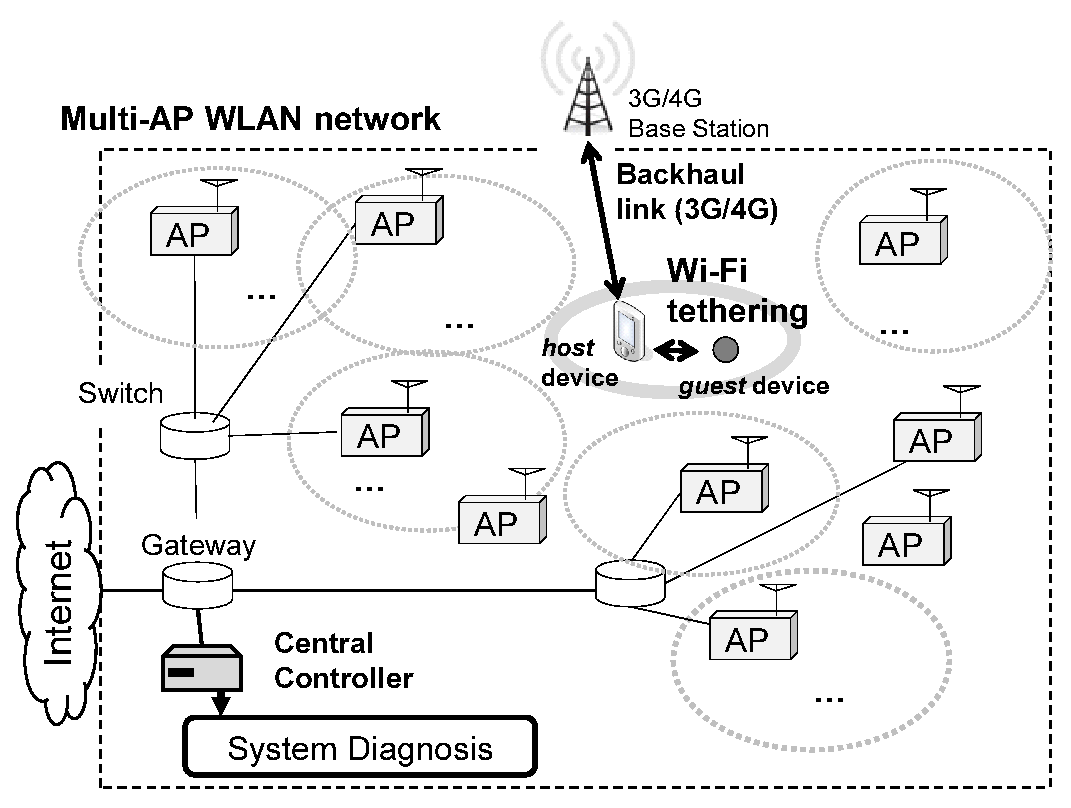
\includegraphics{./figures/FIG_architecure.eps}}
 \caption{Illustration of the problem: selfish misconfigured Wi-Fi tethering
 sets up the network in a centrally managed multi-AP network}
 \label{fig-architecture}
 }
\end{figure}
%
We consider a scenario in which an unauthorized Wi-Fi tethering system
sets up a Wi-Fi hotspot within a centrally managed Wi-Fi network,
where the network consists of a central \emph{controller} and
$N$ 802.11 access points (APs), $A=\{AP_1, AP_2, \cdots, AP_N\}$,
as illustrated in Fig.~\ref{fig-architecture}.
%
%The launched tethering consists of an Internet-connected
The tethering consists of an Internet-connected
(e.g., through 3G/4G cellular connection) mobile phone and a
tethered Wi-Fi-enabled device, contending for channel access
with nearby Wi-Fi systems.
% alex: why do we introduce this metric B_cel here?
Let $B_{cel}$ denote the capacity of the cellular backhaul link.
%
We will henceforth refer to the mobile device and the tethered
Wi-Fi device as \emph{host} and \emph{guest} nodes, respectively;
the \emph{host} node shares its 3G/4G Internet connection
with the \emph{guest} nodes via its Wi-Fi interface.
%

We assume that the multi-AP network is monitored and managed by the
controller, as shown in Fig.~\ref{fig-architecture}. Each $AP_i$
($AP_i \in A$) monitors the channel access activity and reports the
information to the controller periodically.
%
We also assume that frequency planning for each AP in the network
has been done {\em a priori} through a proper channel allocation algorithm
(e.g., \cite{Mishra_MC2R_2005, client_driven06, Mishra_06}), % TODO:add ref
so as to minimize inter-AP inference on each AP.

\subsection{Channel Model}
%
For a given link, let $s$ and $r$ denote the transmitter node
and its corresponding receiver node of a link, respectively.
The distance between the two nodes $s$ and $r$ is
denoted by $d_{s,r}$.
%
We assume that the channel gain $G_{s,r}$ between the transmitter $s$
and the receiver $r$ is determined based on the log-distance
path-loss model described in~\cite{Tse:Viswanath05}:
\begin{equation} \label{eq:pathloss}
G_{s,r} = \frac{1}{{d_{s,r}}^{\alpha}},
\end{equation}
where $\alpha$ is the path-loss exponent (normally, ranging from 2 to 5).
%
Let $P_{s}$ and $P_{r}$ denote the transmission power of node $s$
and the received power at $r$, respectively.
We assume that all the transmitters transmit frames at the same
nominal power $P_{0}$.
%
Then, $P_{r}$ is expressed as $P_{r}=G_{s,r}P_{0}$.
%
The received signal to interference ratio (SIR) $SIR_{r}$
at the receiver is expressed as
\begin{equation}
SIR_{r} = \frac{G_{s,r}P_{0}}{\sum_{k\neq i}{G_{k, r}P_{0}}}.
\end{equation}

Let $\gamma_{m}$ denote the minimum SIR requirement (i.e., SIR threshold)
for successful reception at a receiver node under modulation
scheme $m$, where we consider multi-rate MAC as in 802.11a/b/g/n.

%% [TODO:] .. Error Probability..

%\subsection{802.11 MAC Protocol}

% alex-start
\subsection{Capture Model}
%\emph{Capture Model:}
% alex-end
%
Even when multiple independent transmissions occur simultaneously
to a receiver, the receiver can successfully capture the signal of
interest (SoI) if the received SIR is higher than a certain SIR
threshold, which is known as the {\em capture effect}~\cite{jlee:ychoi07}.

There are two well-known concurrent transmission technologies:
PHY capture effect~\cite{capture} and message-in-message (MIM)
\cite{jlee:ychoi07, MIM}.
Fig.~\ref{fig:capture} illustrates the main difference between PHY
capture and MIM.
%
%
\begin{figure} [t]
\center
  \subfigure[PHY capture effect]{
      \scalebox{0.45}{
      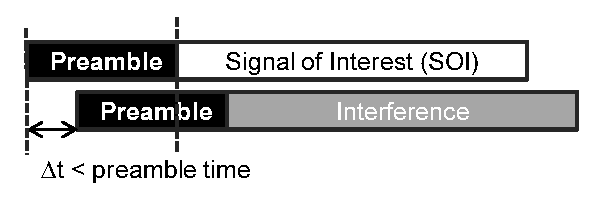
\includegraphics[trim=0.0cm 0.25cm 0.0cm 0.0cm]{./figures/FIG_capture_a_PHY}}
      }\\
  \subfigure[MIM (Message-In-Message)]{
      \scalebox{0.45}{
       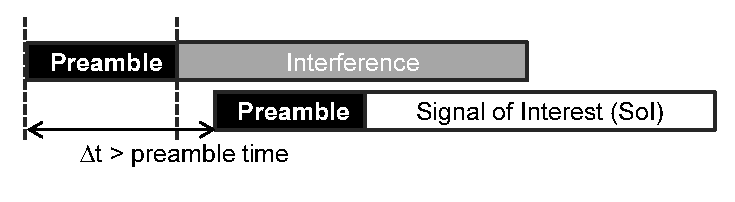
\includegraphics[trim=0.0cm 0.25cm 0.0cm 0.0cm]{./figures/FIG_capture_b_MIM}}
       }
  \subfigure[Adversary Model]{
      \scalebox{0.45}{ \label{fig:capture_c}
       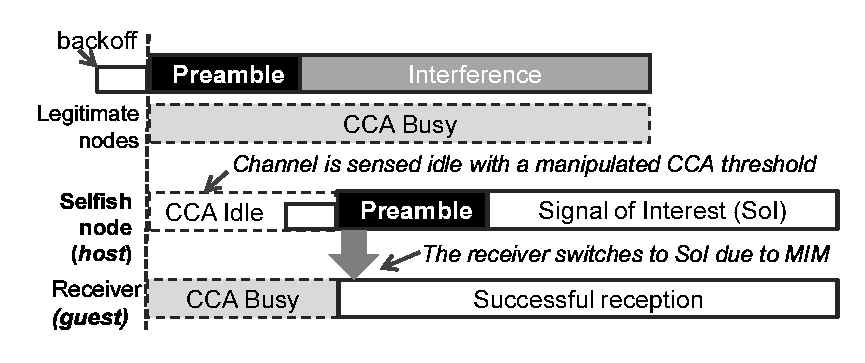
\includegraphics[trim=0.0cm 0.25cm 0.0cm 0.0cm]{./figures/FIG_capture_c_MIM}}
  }
  \caption{(a) PHY capture effect allows a receiver to successfully capture
    the signal of interest (SoI) if its Tx power is sufficiently higher
    than the sum of interferences. (b) MIM (Message-In-Message) allows
    a receiver to disengage from an ongoing packet reception, and
    engage in a new, stronger packet. (c) Selfish behavior with CCA manipulation exploits
    the benefits of MIM if the selfish pair (e.g., tethering link) has a short link distance.}
    \label{fig:capture}
\end{figure}
%
%
The PHY capture effect is the property of 802.11 radios, where
an SoI can be decoded successfully even when the interference arrives
at the same time, as long as the overlap \emph{within} the preamble
detection stage and the SoI is stronger than a specific threshold,
which we call the \emph{capture threshold}.
%
MIM is an enhanced PHY-layer capability that enables a receiver to
decode an SoI even if the SoI arrives after the preamble time of
the interference.
%
Specifically, MIM allows a receiver to disengage from the current
on-going frame reception and re-engage in a new, stronger frame.
However, MIM requires a higher SIR than the PHY capture, which we call
this SIR value the \emph{MIM threshold}, $\beta_{m}$, for modulation
scheme $m$.
%
These capture and MIM thresholds can vary~\cite{Ware:Dut00,
jlee:ychoi07}, particularly depending on the modulation
scheme~\cite{jlee:ychoi07}.

Throughput the paper, we assume that a receiver can decode a frame
successfully with probability greater than 0.9 when the received
SINR is consistently above the SIR threshold for a given modulation scheme.
%
We use the experimental results in~\cite{jlee:ychoi07} to configure
the SIR threshold $\gamma_{m}$ and MIM threshold $\beta_{m}$ for
modulation scheme $m$ (e.g., $m$=BPSK, QPSK, 16QAM, and 64QAM), which
satisfy the requirement of achieving the 90\,\% frame reception ratio.


%\emph{Adversary model :}
\subsection{Adversary Model}
%
We assume that an adversary user manipulates the CCA threshold of the
\emph{host} node's Wi-Fi interface in the tethering while the guest
device is legitimate.
%
We assume that the \emph{host} node selects the maximum possible
CCA threshold without losing the tethering connectivity, which
is likely a little lower than the observed strength of received
signals transmitted by the guest node.
%
In addition, we assume that the adversary user minimizes the link
distance as much as possible so as to exploit the benefits of
physical-layer concurrent transmission technologies, i.e., PHY capture
effect and MIM.
%
Recall a property of Wi-Fi tethering: in general, a tethered hotspot
is formed for communication between personally owned devices which
are placed close-by while in use, and thus the link distance between the
communicating devices is highly \emph{controllable} and typically short
(less than 10\,m or 30\,ft~\cite{Choi:Shin11}).

As shown in Fig.~\ref{fig:capture_c}, the selfish tethering can thus gain exclusive
channel access opportunities, while guaranteeing successful packet
delivery. On the other hand, the legitimate Wi-Fi nodes in the
vicinity will suffer from severe packet corruptions due to the
transmissions from the selfish tethering.

%Our goal is to design an effective mechanism that detects a selfish
%tethering in a multi-AP network.

%!TEX root = info-main.tex
\section{Selfish Configuration in Wi-Fi Tethering}
\label{sec:channel-selection}

%%\subsection{Impact of Selfish Configuration in Wi-Fi Tethering}

To understand the impact of the selfish behavior of a Wi-Fi
tethering system using CCA tuning, we performed extensive simulations
with different transport-layer protocols (i.e., TCP and UDP,
in multi-AP environments) using the ns-2 simulator~\cite{NS2}.

%
\begin{figure} [t]
\center
  \subfigure[Topology-1]{  \label{fig-stopo1}
      \resizebox{26mm}{!}{
      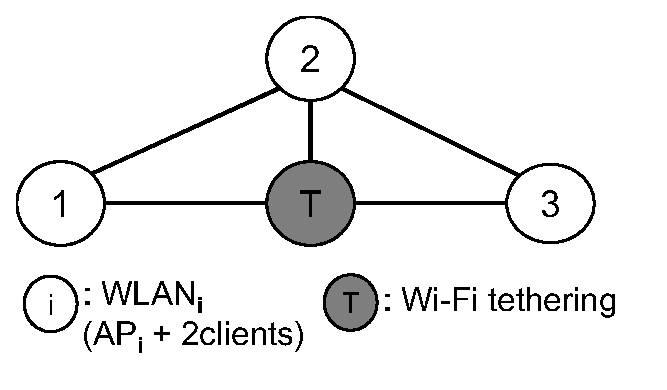
\includegraphics[]{./figures/FIG_sim_topo1}}
      }
  \subfigure[Topology-2]{ \label{fig-stopo2}
      \resizebox{30mm}{!}{
       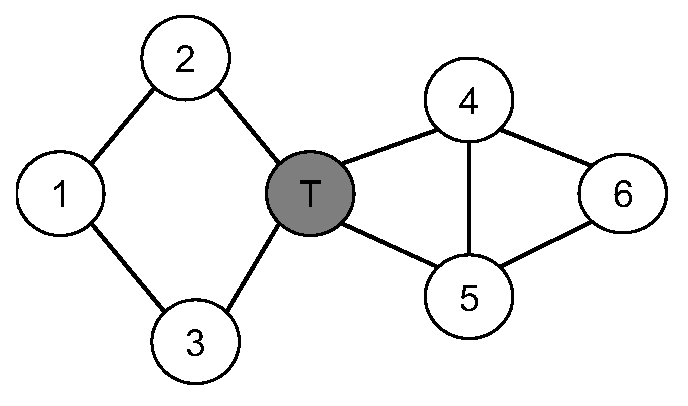
\includegraphics[]{./figures/FIG_sim_topo2}}
       }
    \caption{AP Interference graph of two simulated topologies.}
    \label{fig:sim_topology1}
\end{figure}
%
%
\begin{figure} [t]
  \subfigure[Topology-1, UDP]{  \label{fig-motive-udp-s1}
      \resizebox{40mm}{!}{
      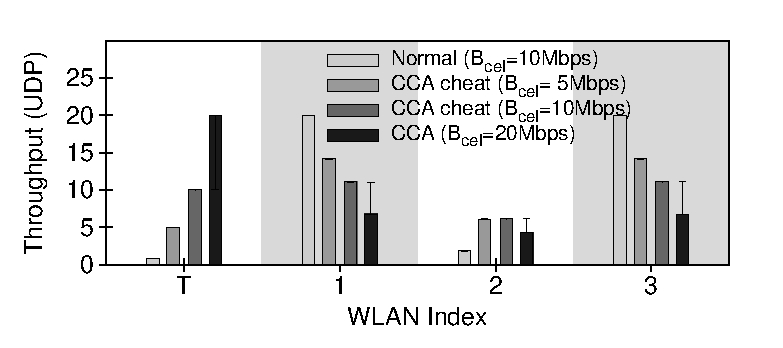
\includegraphics[]{./figures/sim-motive-udp-M1}}
      }
  \subfigure[Topology-1, TCP]{ \label{fig-motive-tcp-s1}
      \resizebox{40mm}{!}{
       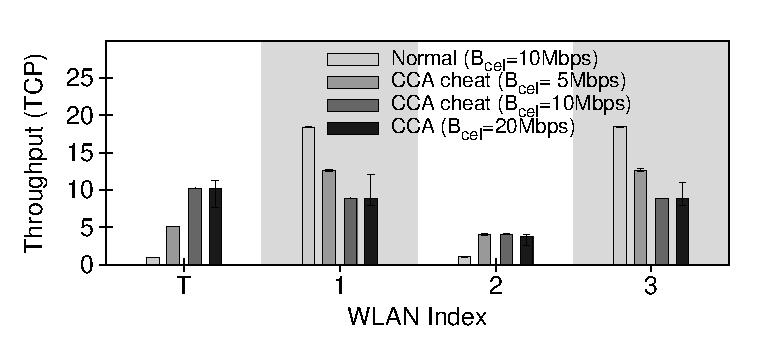
\includegraphics[]{./figures/sim-motive-tcp-M1}}
       }\\
       \subfigure[Topology-2, UDP]{  \label{fig-motive-udp-s2}
      \resizebox{40mm}{!}{
      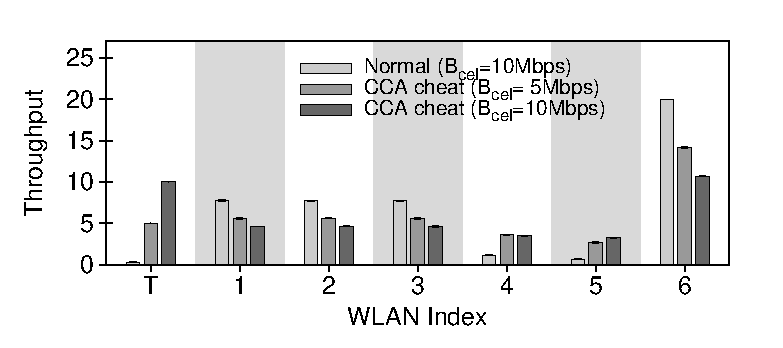
\includegraphics[]{./figures/sim-motive-udp-M2}}
      }
  \subfigure[Topology-2, TCP]{ \label{fig-motive-tcp-s3}
      \resizebox{40mm}{!}{
      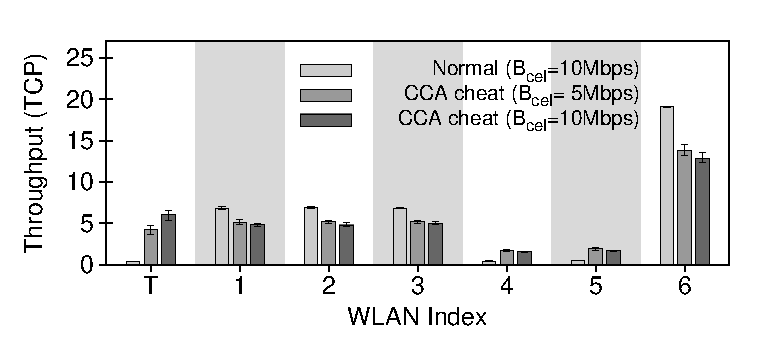
\includegraphics[]{./figures/sim-motive-tcp-M2}}
      }
\caption{Impact of selfish carrier sense on throughput of
transport-layer protocols over various cellular backhaul
link capacities $B_{cel}$ for tethering in two multi-AP topologies.}
    \label{fig:motive-ret1}
\end{figure}
%

\textbf{Multi-AP Topology}:
%
First, we study the impact when a selfish tethering launches within
a well-planned multi-AP network with two representative topologies.
%
The topologies used in the simulations are shown in
Fig.~\ref{fig:sim_topology1}.\footnote{We sampled the topologies from
a popular Wi-Fi database~\emph{Wigle}. For example, the topology shown
in Fig.~\ref{fig-stopo1} corresponds to the well-known FIM
(Flow-In-the-Middle) topology~\cite{FIM08}, which can be easily found
in real-world AP deployments~\cite{choi:shin12}. An edge in the
figure represents the neighboring interference, meaning that an AP is
in the carrier sensing range of its connected APs. The vertex denoted
by `T' in the figure represents the tethering system launched within
the network.}
%

We compare the performance for two cases using UDP and TCP protocols:
(i) \emph{Normal} scenario in which the \emph{host} node uses
the default CCA threshold, and (ii) \emph{Selfish} scenario in
which the \emph{host} node manipulates the MAC protocol by increasing
the CCA threshold as high as possible without losing the connectivity
to the guest.
%
We used the following settings in our simulations.
Each WLAN has an AP and two associated client nodes (i.e., 2 AP--clients
flows per WLAN), and all nodes operate on the same channel.
We considered typical IEEE 802.11a/g MAC/PHY parameters with the
maximum speed of 54\,Mbps, and set the capacity $B_{cel}$ of
the 3G/4G backhaul link of tethering to 5, 10, and 20\,Mbps.
Traffic is generated by a constant bit rate (CBR) traffic generator
for the UDP protocol (1\,KB packet size), and an FTP download
application is used to create TCP flows (1.5\,KB packet size).
% alex: the UDP traffic scenarios is not clear to me.
For UDP flows, we assume 10\,Mbps for flows in infrastructure APs,
and 20\,Mbps for tethering flows.


Fig.~\ref{fig:motive-ret1} shows the throughput of the tethering link
and APs. In \emph{Normal} case, we can see a throughput imbalance
among APs, and especially, the tethering flow is shown to experience
starvation due to the FIM problem~\cite{FIM08}.
%
With the CCA cheating, on the other hand, we can see that the
selfish tethering achieves a significant throughput gain at the cost
of significant throughput degradation for other nearby well-behaving
APs, for both UDP and TCP flows.
%
%Note that TCP is a bidirectional transfer-based protocol and
%here the CCA function is manipulated only on the host side,
%i.e., the \emph{guest} node is legitimate.
%
%Nevertheless, the selfish tethering achieves a high throughput gain
%with the TCP protocol.
%
Although we manipulate the CCA threshold only on the host side,
i.e., the \emph{guest} node is legitimate, the selfish tethering
achieves a high throughput gain even with the TCP protocol,
which is a bi-directional, transfer-based protocol.
%
This is attributed to the closed-loop TCP-ACK mechanism, i.e., the
more data packets (or ACKs) the legitimate guest successfully receives
from the misconfigured host, the more outstanding uplink ACKs (or data
packets) the guest can transmit.
%
% alex: what would be the toughput impact if we manipulate the CCA
% threshold from the guest node, more or less throughput gain?
The figure shows that the throughput gain increases proportional to
the cellular backhaul link bandwidth, $B_{cel}$, for both UDP and TCP
flows.


One can expect that selfish CCA manipulation would increase the
collision probability of the tethering link since the \emph{host}
node initiates packet transmission even in the present of other
nodes' transmissions. Nevertheless, we observe a significant gain
of selfish behavior using CCA manipulation, as seen from the above results.
%
To understand why the selfish tethering link can achieve a significant
gain with CCA manipulation, we investigate the property of the
successful receptions at the tethering receiver node, i.e.,
\emph{guest} node.
%
Table~II plots the collision probability, and the percentage of
successful receptions at the receiver in the simulation
with $B_{cell}$=10\,Mbps corresponding to the results shown
in Figs.~\ref{fig-motive-udp-s1} and \ref{fig-motive-udp-s2}, respectively.
We observe that, despite the high collision ratios (71.5\,\% and 91.8\,\%
for Topology 1 and 2, respectively), the tethered receiver can capture
the signal of interest (SoI), thanks to PHY capture effect and MIM.
A majority of the successful receptions are due to MIM, i.e., 63.6\,\%
and 63.5\,\% for Topology 1 and 2, respectively.
Note that the link distances between \emph{host} and \emph{guest}
nodes are very short, making the received signal at the \emph{guest}
node sufficiently stronger than the sum of interferences.

\begin{table}[ht]\label{table:ratio}
\renewcommand{\arraystretch}{1.2}
\caption{Statistics of receptions at the receiver (in case of UDP
and $B_{cell}$=10\,Mbps}
\vspace{-0.2cm}
\centering
\begin{tabular}{|c|c c c |}
\hline \bfseries Topology & Collision prob. & Capture effect & MIM\\
\hline\hline
1 & 71.5 & 17.9 & 63.6 \\
\hline
2 & 91.8 & 28.3 & 63.5 \\
\hline
\end{tabular}\label{tbl:txdist}
\end{table}

These results clearly demonstrate that the selfish behavior using CCA
manipulation abuses the short link distance property of Wi-Fi
tethering and thus makes it possible to exploit the benefits of MIM.
Consequently, the selfish tethering can achieve an unfair throughput
gain regardless of the network condition surrounding the tethering.

\begin{figure} [t]
\center
  \subfigure[Scenario 1]{  \label{fig-patialCH_a}
      \resizebox{24mm}{!}{
      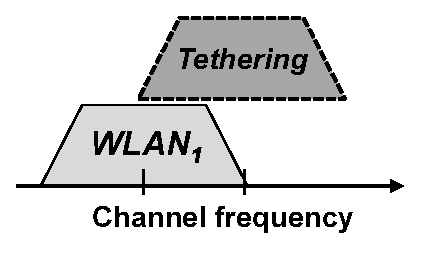
\includegraphics[trim=0.0cm 0.25cm 0.0cm 0.0cm]{./figures/FIG_motive_topo_1a}}
      }
  \subfigure[Scenario 2]{ \label{fig-patialCH_b}
      \resizebox{31mm}{!}{
       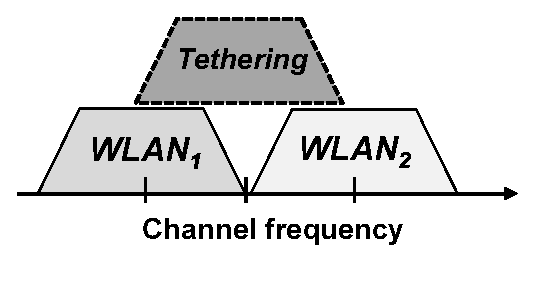
\includegraphics[trim=0.0cm 0.25cm 0.0cm 0.0cm]{./figures/FIG_motive_topo_1b}}
       }\\
  \subfigure[Throughput for Scenario 1]{  \label{fig-ret_patialCH_a}
      \resizebox{40mm}{!}{
      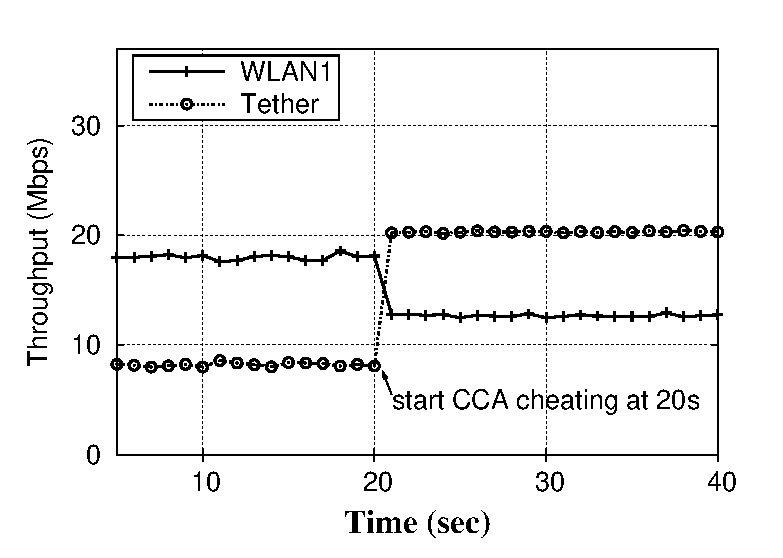
\includegraphics[trim=0.0cm 0.25cm 0.0cm 0.0cm]{./figures/FIG_sim-motiveA_24M}}
      }
  \subfigure[Throughput for Scenario 2]{ \label{fig-ret_patialCH_b}
      \resizebox{40mm}{!}{
       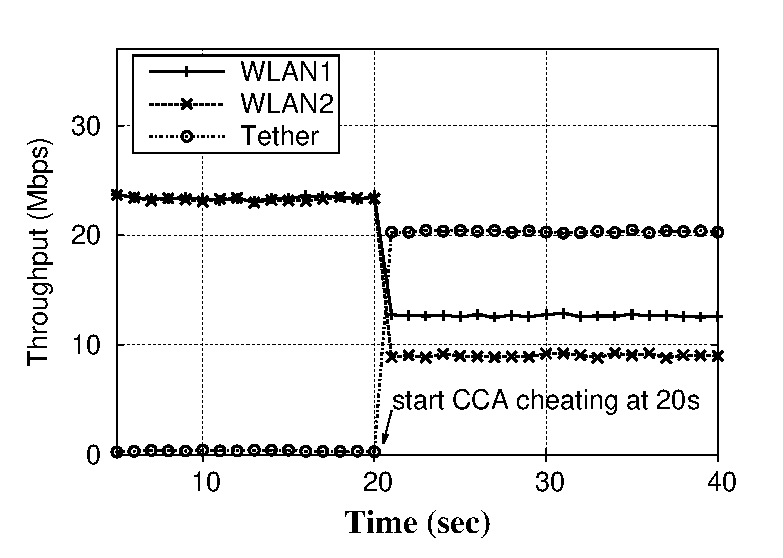
\includegraphics[trim=0.0cm 0.25cm 0.0cm 0.0cm]{./figures/FIG_sim-motiveB_24M}}
       }
    \caption{Impact of launching tethering on a partial-overlapped channel.}
    \label{fig:motive_A}
\end{figure}


%
\textbf{Impact of Tethering Channel}:
%
Next, we study the impact of the CCA manipulation on performance
when tethering is launched on a channel partially overlapping
with nearby APs. As mentioned above,
the tethered Wi-Fi hotspot can potentially set up the network with
an \emph{arbitrary} channel number, which may cause serious interference
to nearby well-planned APs.
We used two simple scenarios in \cite{zhang:shin11icnp} and the
channel model presented in \cite{Mishra:Arbaugh05} for our simulation.
Fig.~\ref{fig-patialCH_a} illustrates a simple case that the channel
selected by the tethering is partially overlapping with a nearby AP.
Since two overlapping channels are sensed by each other by the CCA
mechanism of 802.11, its effective spectrum usage is
only 20\,MHz \cite{zhang:shin11icnp}.
%
Fig.~\ref{fig-patialCH_b} depicts the case when the tethering shares
the spectrum with two adjacent orthogonal channels.
Note that in this case, the tethering link may suffer from channel
starvation \cite{zhang:shin11icnp}; the tethering link can transmit
only when both $WLAN_1$ and $WLAN_2$ are idle, but the probability of
the two outer channels being idle at the same time is very low
because the channel activities on the two outer channels are
asynchronous and may overlap randomly.

To evaluate the impact of the selfish behavior using CCA manipulation
in these scenarios, we performed simulations with following setting.
Each WLAN consists of two client nodes where the traffic on each flow
is generated with 10\,Mbps downlink CBR over UDP.
The capacity $B_{cel}$ for tethering is configured to 20\,Mbps
(with 20\,Mbps CBR/UDP traffic).
Initially, the tethering link is set to be legitimate.
The CCA manipulation is activated at 20\,s.

Figs.~\ref{fig-ret_patialCH_a} and \ref{fig-ret_patialCH_b} plot
the resulting throughput showing the effect of selfish behavior
using CCA manipulation.
When the tethering is legitimate, it achieves a fair share of shared
medium with two flows in $WLAN_1$ in the first scenario.
In the second case shown in Fig.~\ref{fig-patialCH_b},
the tethering is almost starved due to the channel starvation
problem \cite{zhang:shin11icnp}.
After the CCA value is configured selfishly,
despite the same unfair channel condition,
the tethering link achieves a significant throughput gain
at the cost of significant reduction in throughput of other flows.

In the same scenario depicted in Fig.~\ref{fig-patialCH_b},
we also compare the impact of CCA manipulation with
different types of selfish behavior manipulating other MAC parameters,
in particular manipulation of the backff mechanism using
smaller values of $CW_{min}$.\footnote{The manipulation of backoff mechanism
is widely adopted by selfish users~\cite{K:Vaidya05}.}
%
Fig.~\ref{fig:cwmin_cheat} shows the simulation results
with different values of $CW_{min}=$31,\,15,\,7,\,and 3.
%
The figure indicates that the selfish behavior using CCA manipulation
achieves throughput gain above those with smaller values of $CW_{min}$
and even higher than very aggressive setting with $CW_{min}=3$.
%
The results imply that the manipulation of CCA threshold is a simple,
yet more attractive approach that can be abused by adversaries in
a tethering environment.

\begin{figure} [ht]
\center
  \subfigure[2~client~nodes~per~WLAN]{ \label{fig-udp-10AP}
      \resizebox{33mm}{!}{
       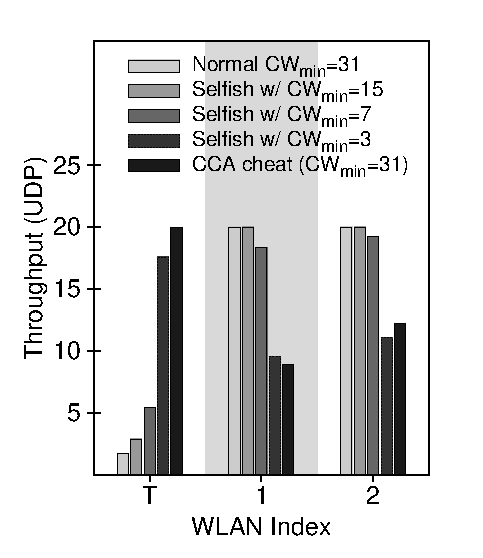
\includegraphics[trim=0.5cm 0.25cm 0.5cm 0.25cm]{./figures/sim-comp_cw_N2}}
       }
       \subfigure[5~client~nodes~per~WLAN]{  \label{fig-tcp-10AP_downlink}
      \resizebox{33mm}{!}{
      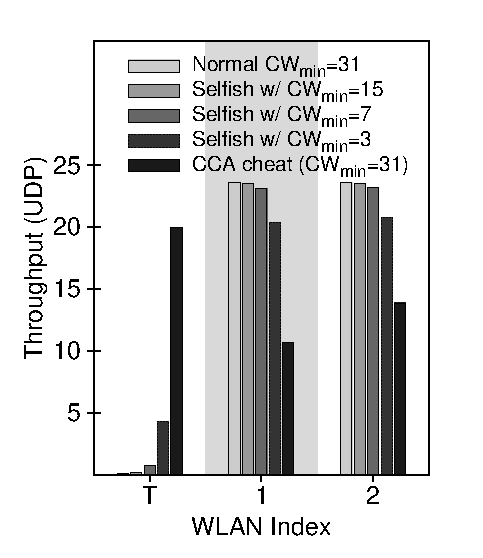
\includegraphics[trim=0.5cm 0.25cm 0.5cm 0.25cm]{./figures/sim-comp_cw_N5}}
      }
    \caption{Throughput comparison with selfish configurations of the $CW_{min}$ parameter.}
    \label{fig:cwmin_cheat}
\end{figure}


%
\textbf{Impact of Cellular Backhaul Link Capacity}:
%
Finally, we evaluate the impact of the backhaul link capacity of
selfish tethering.
%
\begin{figure} [ht]
 \center{
        \scalebox{0.55}{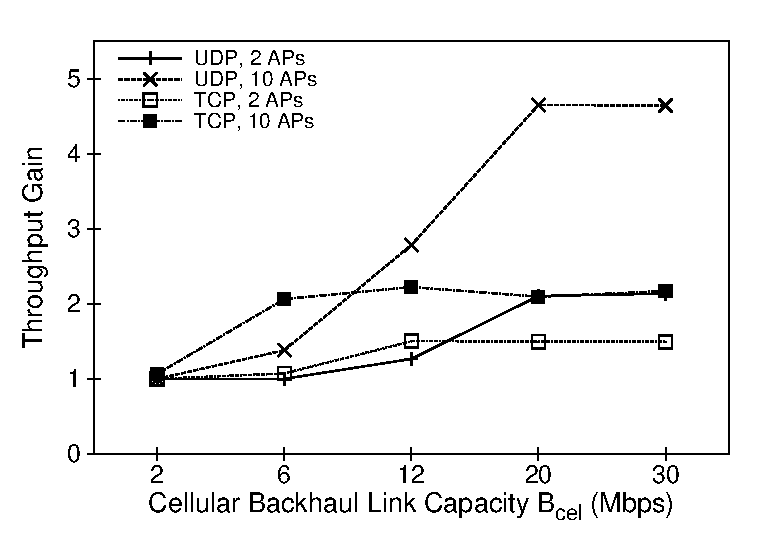
\includegraphics{./figures/sim-sel-gain}}
       }
    \caption{Throughput gain of selfish carrier sensing over
various cellular backhaul link capacities and AP densities.}
    \label{fig:throughput-gain}
\end{figure}
%
Fig.~\ref{fig:throughput-gain} shows the throughput gain of the selfish
behavior as a function of backhaul link capacity for TCP and UDP
downlink traffic in a network with a high density of APs consisting
of 10 APs and 30 client nodes.
The figure indicates that the throughput gain is proportional to the
backhaul link capacity of the maximum achievable goodput determined
by the transport-layer protocol.\footnote{Note that in our simulation
when the backhaul apacity is larger than 20\,Mbps, the maximum
throughput is bounded by the Wi-Fi link capacity in this simulation.}
This is because the higher backhaul link capacity the tethering is
connected to, the more outstanding packets the selfish node can transmit.

%%
%% we will not include the following subsection this time
%%
\comment {%%%%%%%%%%%%%%%%%%%%%%%%%%%%%%%%%%%%%%%%%%%%%%%%%%
%
%
%
% COMMENT..

\subsection{Best Strategy of Selfish Tethering Nodes}

  %      [MIM Capture Effect]

For an adversary, the best selfish strategy is to increase the CCA
threshold as much as possible in order to increase his own throughput.


 %%  TODO: 아래 문구 수정. as much as possible
We now analytically show that, in tethering environments where
the link distance between host and guest devices is adjustable, a
selfish node can gain exclusive channel access while guaranteeing
a target frame reception ratio.
%
To derive the best strategy for the selfish node, we first need to
compute the throughput capacity of the tethered link.

Let $\theta_{s}$ denote the CCA threshold of node $s$ above which
node $s$ can correctly sense the symbols, and thus does not transmit
and freezes its backoff process \cite{ieee:80211-07}.
%
For given node $s$, we define the carrier sense set $C_{s}( \theta_{s} )$
as
%
\begin{equation} \label{eq:set_c}
C_{s} (\theta_s)= \{ k | G_{k, s} P_{0} > \theta_{s} \}.
\end{equation}
%
The nominal CCA threshold adopted by all legitimate nodes in the network
is denoted by $\theta_{0}$. By definition, for $\theta_s\!\geq\!\theta_{0}$,
$C_{s} (\theta_s) \! \subset C_{s}( \theta_0 )$.

From Eqs.~\eqref{eq:pathloss} and \eqref{eq:set_c},
the carrier sensing range, denoted by $R_{cs}$, is determined by the
CCA threshold, as:
\begin{equation}
R_{cs}(\theta) \! = \Big(\frac{ P_0 }{\theta} \Big)^{1/\alpha}.
\end{equation}

We consider 802.11g/n PHY which employs multiple modulation and
multiple coding schemes (MCSs) \cite{IEEE802.11n},
where the MCS schemes are listed in Table~I. %%%
%
%
Let $\gamma_{m}$ denote the minimum SIR requirement
(i.e., SIR threshold) for the successful reception at a receiver node
for each MCS scheme $m$.
%
Hence, for a transmission of node $s$ at MCS scheme $m$,
let $I_{r,m}$ be the \emph{interference set}  of nodes whose
simultaneous transmission will prevent node $r$ from correctly
decoding the frame from $s$:
\begin{equation}
I_{r, m} = \{ k | G_{k, r} P_{0} > \frac{ P_r }{ \gamma_{m} } \}.
\end{equation}

Hence, for a given MCS $m$, an interference occurs at receiver $r$ if
any node in $I_{r,m}$ transmits data simultaneously with transmitter $s$.

From the perspective of the sending node of an 802.11 link $i$
whose transmitter and receiver are denoted by $s$ and $r$, respectively,
the link's activity can be characterized with the following
three different channel states \cite{Gao:06}:
(a) \emph{self channel} occupied by the node's own transmission,
(b) \emph{busy channel} due to the activity of other neighboring nodes,
and (c) \emph{idle channel} when the channel is not used by any node.
%
Let ${x}_i(\theta_s)$, ${y}_{i}(\theta_s)$, and ${z}_{i}(\theta_s)$
denote, respectively, the fraction of time link $i$ stays in these
three states.
%
These variables are determined by the PHY- and MAC-layer
behavior of nearby 802.11 links, including link $i$
and neighboring links, with CCA threshold $\theta$.

Let $p_i(\theta_s)$ be the conditional transmission error
probability\footnote{The probability of an error seen by
a packet being transmitted at the receiver.} of link $i$,
given that a transmission attempt is made, which can be expressed:
\begin{eqnarray}
p(\theta_s)=&P[\text{simultaneous TX in }C_{r}(\theta_s)]\!\cdot\
\!P[\text{not capture effect}] \nonumber \\
&+ P[\text{no TX in }C_{r}(\theta_s)]\!\cdot\
\!P[\text{TX in }I_{r}],
\end{eqnarray}
where $TX$ is an abbreviation for transmission.
%
Then, the available throughput capacity $S_i(\theta)$ of link $i$
with CCA threshold $\theta_s$ is given by
\begin{equation}
S_i(\theta_s) = {x}_i(\theta_s) \times \Big(1 - p_i(\theta_s)\Big) \times R_i \times
\frac{T_{payload}}{T_{tx}},
\end{equation}
where $R_i$ is the data transmission rate, $T_{payload}$ is the
average transmission time of the data payload, and
$T_{tx} = T_{Header} + T_{payload}+ SIFS + (Block)ACK + DIFS $
is the average overall transmission time (in number of time slots) for
a packet, including PHY and MAC headers, data payload and ACK, as well
as DCF Inter-frame Space (DIFS) and Shortest Inter-frame Space (SIFS).
Since we are only interested in the \emph{maximum} available
capacity of link $i$, we assume that the node always has
backlogged packets to transmit.

In 802.11 MAC, nodes attempt to transmit only during an idle slot.
In other words, the sender node counts down its backoff timer
to transmit a packet only during idle periods, and it defers the
count-down process whenever the channel is sensed busy.
Thus, if we let $\tau(p)$ model the attempt rate per idle slot for
a given transmission-error probability $p$ \cite{Kumar:07Fixed},
then the normalized self airtime ${X}_i(c)$ is proportional to
the normalized idle-time ${Z}_i(c)$ and can be expressed as:
\begin{equation}
{x}_i(\theta) = {z}_i(\theta) \times \tau\big(p_i(\theta)\big) \times T_{tx}.
\end{equation}
%
Therefore, we obtain the throughput capacity $S_i(\theta)$ of link $i$
on channel $c$ as
\begin{equation}\label{eq:linkcapacity}
S_i(\theta) =  {z}_i(\theta) \times \tau\big(p_i(\theta)\big) \times \Big(1 - p_i(\theta)\Big)
\times R_i \times T_{payload}.
\end{equation}
%
Note that the data rate $R_i$ is determined by the
physical link condition of link $i$.
%%---1

Based on the above equation showing the relation between the throughput
of a link ad its CCA threshold $\theta$, we have the following proposition.

\begin{proposition}[Proposition 1]
When the link distance is less than a certain value, by manipulating
the CCA threshold, a selfish node can gain exclusive channel access
without reducing the frame reception ratio.
\end{proposition}
%\vspace{0.15cm}
\begin{proof}
%%
%%
See Appendix A.
\end{proof}
%%

Thus, an adversary user can  gain exclusive channel access in
tethering environments where the link distance between the host and
guest devices is controllable to gain an unfair advantage in
throughput performance by manipulating the tethering function.
For example, by rooting or jailbreaking mobile OSes, the channel
access functions of Wi-Fi protocol can be manipulated ``selfishly,''
at the cost of other nearby well-behaving Wi-Fi devices' performance.
Therefore, detecting unauthorized and misconfigured tethering Wi-Fi
is becoming a very important task in most organizations.

} %%%% COMMENT

%!TEX root = info-main.tex
%%% Section IV
\section{Detection Architecture in a Multi-AP Network}

In this section, we first identify the key features of selfish
carrier sensing behavior. We then propose an online detection
architecture, called {\tt CUBIA}, that diagnoses the network
condition in a multi-AP network, consisting of (i) a \emph{AP-level
diagnosis} stage and (ii) a \emph{system-level reaction} stage.
%
In what follows, we will detail the design of this architecture.


\subsection{Key Feature of Selfish Carrier Sense Behavior}

Selfish carrier sensing on a tethered host node may result in
excessive frame loss of nearby legitimate APs, and thus, successful
detection of selfish misbehavior depend largely on a AP's ability
of identifying the root cause of its frame losses.
%
In 802.11 WLANs, there are four main causes of frame losses:
(i) PHY-layer link quality degradation, (ii) MAC-layer collision,
(iii) hidden nodes, and (iv) selfish nodes (e.g., manipulation
of the CCA thresholds).

Fortunately, selfish tethering exhibits unique features that
can help distinguishing the selfish carrier sensing of a
tethering host from other causes of frame losses, especially
from the hidden node problem.
%
We made the following two observations:

\myitemizebegin
%
\item[{\bf O1)}]
While the victim nodes of the selfish tethering experience
symptoms similar to those of the \emph{hidden node problem}
(i.e., transmissions of the legitimate node are continuously
corrupted by the selfish node), the victim nodes' communications
cannot be fully protected by the Request-to-Send/Clear-to-Send
(RTS/CTS) exchange mechanism, i.e., a virtual carrier sensing,
because the selfish node may not recognize (due to its short
communication range) or respect the RTS/CTS frames.
%
%Unlike the hidden node problem, however, remedies are different.
%That is, the hidden node problem can be mitigated by the
%Request-to-Send/Clear-to-Send (RTS/CTS) exchange, i.e., the virtual
%carrier sensing mechanism, but the selfish carrier sensing problem cannot,
%because the RTS/CTS frames are not recognized/respected by the selfish
%node due to its short communication range.
%
\item[{\bf O2)}]
When selfish tethering exists, the victim nodes may suffer from
increased number of frame losses, hence throughput degradation,
because the selfish tethering initiates a transmission even when
the victim nodes have already been transmitting packets.
%
In a multi-AP network, majority of nearby APs will likely to
experience the similar severe packet errors simultaneously when
the selfish tethering is present. In contrast, the impact of the
hidden node problem is limited to the nodes in the hidden area.
%
\myitemizeend


\subsection{CUBIA: A Proposed Selfish Diagnosis Algorithm}

Based on the above observations, we propose a simple, yet efficient
online detection algorithm at each AP, which can accurately distinguish
the selfish behavior with CCA manipulation from other types of network
problems, such as severe network congestion (i.e., collisions) and
the hidden node problem.

\subsubsection{Diagnosis Stage}
%
The first diagnosis stage is to infer the asymmetric carrier sensing
condition at each AP in the network. Based on above observations,
we propose a simple interference inference algorithm, called {\tt CUBIA}
({\em Two-Phase CUsum-Based Interference inference with Adaptive RTS/CTS}).
%
%By exploiting the above observation on the unique feature of selfish
%misbehavior using CCA manipulation, we propose a simple interference
%inference algorithm, so called CUBIA ({\em Two-Phase CUsum-Based
%Interference inference with Adaptive RTS/CTS}).
%
{\tt CUBIA} runs at each AP and it diagnoses the network condition by passively
monitoring the ongoing traffic with its client nodes.
%
Specifically, if {\tt CUBIA} detects severe and persistent frame transmission
failures, it employs the RTS/CTS exchange before each data transmission
to rule out the possibility of the hidden node problem.
%
%differentiate the hidden node problem from frame transmission failures
%by the selfish carrier sensing.
%
For this, {\tt CUBIA} employs the CUSUM (CUmulative SUM) algorithm~\cite{Gustafsson:2000}
to quantify the duration of frame losses. CUSUM algorithm suits our needs
because it is simple and light-weight, and it has been widely used for the
detection of state changes. We will elaborate the detailed procedure of
the detection mechanism using CUSUM algorithm.

%As mentioned earlier, unlike the hidden node problem,
%a data transmission following a successful RTS/CTS exchange
%is not protected in the presence of a selfish node.
%The heart of CUBIA algorithm is that,
%to quantify how long the corruption lasts, it adopts the CUSUM
%(CUmulative SUM) algorithm~\cite{Gustafsson:2000}, which has been
%widely used for the detection of state changes.
%
% Jaehyuk: Due to the lack of 80211n node in simulation tools,
%                   I changed the algorithm that is available in ns-2
%
%In particular, the AP exploits the frame aggregation and
%block ACK mechanism in the 802.11 to diagnose the cause of
%frame losses~\cite{ieee:80211e, ieee:80211n}.
%
%Frame aggregation is a feature of the IEEE 802.11e and 802.11n standards,
%designed to increase throughput by sending two or more data frames
%in a single transmission~\cite{ieee:80211e, ieee:80211n}.
%%
%802.11e EDCA provides contention-free access to the channel for a period
%called {\em Transmit Opportunity} (TXOP), allowing multiple frames
%to be transmitted in a single TXOP.
%%
%The 802.11n standard allows MAC Protocol Data Unit (MPDU) aggregation,
%called A-MPDU, whereby multiple subframes are packed into
%a single aggregated frame.
%%
%Block acknowledgments (block ACKs) allow an entire TXOP and A-MPDU
%to be acknowledged in a single frame, reducing protocol overhead.

%We made the following observation to detect the asymmetric carrier
%sensing condition: in case of asymmetric carrier sensing condition
%like the hidden node problem, the receiver of the ongoing transmission
%of an aggregated frame (e.g., A-MPDU) can suffer from \emph{partial}
%and \emph{bursty} frame losses.
%
%
%%% alex: why this is the case?
%In particular, bit errors are likely to be located after the front
%section of the aggregated transmission, while the front section of the
%transmission has a much lower probability of incurring bit errors
%compared to the rest of the packet.
%
%
%%
%%  [FIGURE]
%%Fig.~X shows the
%%[Experiment results should be here]
%
%Then, the receiver reports the status (i.e., success/failure) of each
%subframe of the A-MPDU frame to the transmitter via a block ACK frame.
%Consequently, the transmitter node can know the result of the
%transmission and calculate the error probability of subframes.

{\tt CUBIA} monitors the frame error rate (FER) for every $m$ transmissions
to detect any abrupt changes in network condition, which might indicate
the possibility of selfish tethering nodes.
%
Let $p_{k}^{i}$ denote the frame error rate for the $k$-th measurement
period at $AP_i$, given by $p_{k}^{i} = e_{k}/m$, where $e_{k}$ denotes
the number of transmission failures. Then, we calculate the average
error probability, $E[p^{i}]$, by a moving average to reflect the
network dynamics as:
%
\begin{equation} \label{Eq:move_avg}
E[p^{i}] = \lambda \cdot E[p^{i}]  + (1 - \lambda) \cdot p_{k}^{i}.
\end{equation}

We define the CUSUM change detection filter $c_k^i$ of $AP_i$ as:
\begin{eqnarray}
&c_k^i = \max(~0, ~c_{k-1}^i + p_{k}^{i} - v~),\label{Eq:CUSUMg} \\
&c_0^i = 0,\nonumber
\end{eqnarray}
where $v$ is a drift parameter, which is a filter design parameter.
$v$ is configured differently according to the value of $c_k^i$ as:
%
\begin{equation}\label{Eq:CUSUMv}
v =
\begin{cases}
E[p^{i}] + \mathcal{T}_{FER},  & \mbox{if } c_k^i < \theta_{AS} \\
\mathcal{T}_{FER}, & \mbox{if } \theta_{AS} \leq  c_k^i \leq \theta_{S},
\end{cases}
\end{equation}
%
where $\theta_{AS}$ and $\theta_{S}$ denote
the {\em first alarm threshold} for asymmetric carrier sensing, and
the {\em second alarm threshold} for inferring selfish carrier sensing,
respectively.

{\tt CUBIA} issues the first alarm to $AP_i$ when $c_k^i > \theta_{AS}$.
Then, {\tt CUBIA} turns on the RTS/CTS exchange mechanism, and
keeps track of the change detection with
$v = \mathcal{T}_{FER}$ in Eq.~\eqref{Eq:CUSUMg}.
%
Note that the first alarm can be caused by
a sudden severe MAC-layer congestion or a hidden node problem.
%
%
However, in such a case,
%i.e., if the first alarm stems from the MAC-layer congestion or
%the hidden terminal problem,
the magnitude of $c_k^i$ tends to decrease with RTC/CTS frames,
because the the collisions are filtered out \cite{CARA} and
the hidden terminal problem are mitigated with RTS/CTS
exchange, and the frame error rate decreases accordingly.

On the other hand, if the first alarm is caused by the selfish carrier
sensing problem, the transmission of a frame transmission following
successful RTS/CTS exchanges will be interfered with, and hence,
 even with RTS/CTS, the magnitude of $c_k^i$ would continue to
increase, even beyond $\theta_{S}$.
%
%
Recall that under the normal condition, PHY-layer link quality is stable
and has a certain upper bound $\mathcal{T}_{FER}$, namely \emph{target}
frame error rate, which is guaranteed by the underlying rate-adaptation
scheme that adjusts the modulation schemes to meet the target
FER.\footnote{For example, practical rate adaptations \cite{Jensen10}
adjust the modulation schemes to meet the target FER (frame error rate),
and thus guarantee the average FER performance to be maintained
around the target value.}

Consequently, $AP_i$ sends a second alarm to the central controller
(see Fig.~\ref{fig-architecture}) if $c_k^i > \theta_{S}$,
which may trigger the \emph{reaction}
to solve the selfish carrier sensing problem.

\subsubsection{Reaction Stage}
%
Although the focus of this paper is to propose an AP-level detection
mechanism, it is important to cope with the selfish misbehavior detected
whin the network at the system level.
% 
%Here, we present a simple decision policy with which the controller
%determines when to take follow-up actions to cope with the selfish
%misbehavior detected whin the network.
% Jaehyuk
Here, we discuss how the controller determines when to take 
follow-up actions to cope with the selfish misbehavior detected 
whin the network.

In typical managed Wi-Fi networks, the information obtained at APs
is integrated on the controller. Then, the controller utilizes
the information to improve the detection accuracy.
%
As explained in observation {\bf O2}, majority of nearby APs will likely 
to experience the similar severe packet errors simultaneously when
the selfish tethering is present. Consequently, the victim APs send
the second alarm to the controller at the same time.
By exploiting the spatial and temporal correlation in those alarms, 
the controller identifies the root of the problem more effectively and 
accurately. 
%
For example, if a certain condition is satisfied,
the controller can take various follow-up actions, which can
be (i) localizing the rogue interfering node~\cite{Joshi:Katti2013},
and (ii) remedying victim APs (e.g., interference-aware channel
reassignment), etc. However, the detailed follow-up actions are
beyond the scope of this paper.

%%%!TEX root = info-main.tex
\section{Performance Evaluation}

We now evaluate the performance of the
proposed detection algorithm via simulation.
We have implemented the proposed {\tt CUBIA} in ns-2
simulator (ver.3.35) \cite{NS2}.

\subsection{Simulation Setup}

%
In the simulation, the multi-AP network is deployed in a $200\times200$
\,$m^2$ area, where 5 APs with 10 client nodes are randomly generated;
this represents a densely-populated configuration fully covering
the entire area.
%
The transmission range and carrier sensing range of legitimate nodes
are set to 75\,m, and 150\,m, respectively. A selfish tethering pair
is placed at the center of the area, whose link distance and carrier
sensing are set to 1\,m and 10\,m, respectively. Table~\ref{table_sim_param}
lists the parameter values used in the simulation study.

\begin{table}[ht]
\renewcommand{\arraystretch}{1.2}
\caption{Parameters used in performance evaluation}
\label{table_sim_param} \centering
\begin{tabular}{|c|c|}
\hline \bfseries Parameter & \bfseries Value \\
\hline
 Transmission range  & 75 \\
 Carrier range       & 150\\
 Data rate / ACK rate & 54\,Mbps / 6\,Mbps \\
 CBR rate per AP-client pair (UDP)& 20\,Mbps \\
 payload size of UDP , TCP& 1000, 1500\,bytes   \\
 $\mathcal{T}_{FER}$ (in Eq.~\eqref{Eq:CUSUMv}) & 0.05 \\
 $\lambda$ (in Eq.~\eqref{Eq:move_avg}) & 0.1\\
 % alex: there is no reference Eq:move_avg
 $m$ & 10\\
 the maximum allowed latency of detection & 2 sec\\
\hline
\end{tabular}
\end{table}

The performance is evaluated in terms of detection accuracy
and time for TCP and UDP protocols. We consider a downlink
scenario where each AP transmits frames to its client nodes.

\begin{figure*} [ht]
\center
  \subfigure[Selfish carrier sensing problem]{  \label{fig-eval-dynamic1}
      \resizebox{55mm}{!}{
      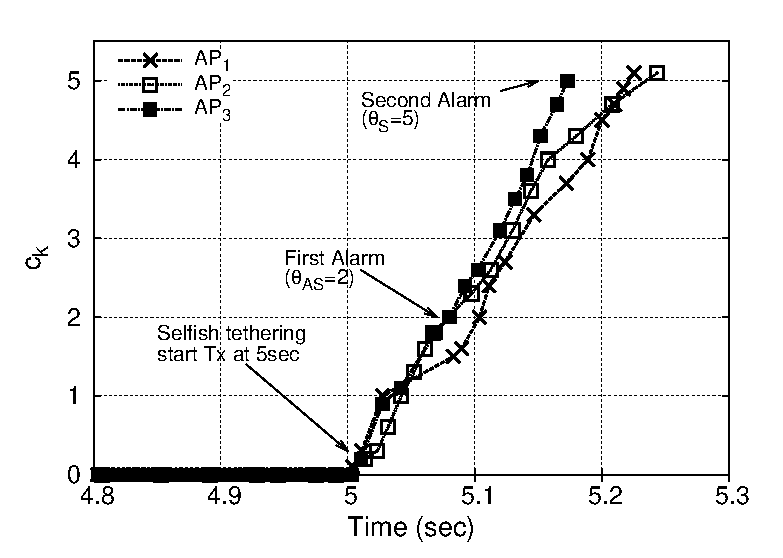
\includegraphics[]{./figures/eval/fig-CUBIA_dynamic-M1_udp}}
      }
  \subfigure[Sudden collisions]{ \label{fig-eval-dynamic2}
      \resizebox{55mm}{!}{
       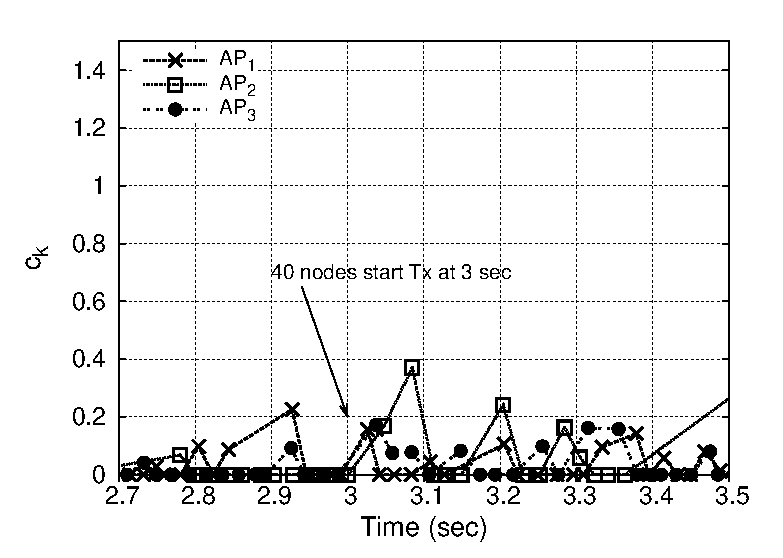
\includegraphics[]{./figures/eval/fig-CUBIA_dynamic-mac}}
       }
       \subfigure[Hidden node problem]{  \label{fig-eval-dynamic3}
\vspace{-0.5cm}
\centering
\epsfxsize=50mm
\epsfbox[50 110 410 402]{./figures/eval/fig-CUBIA_dynamic-hidden}
\vspace{-0.2cm}
      }
\caption{The dynamics of {\tt CUBIA} toward three difference types
of frame losses.}
    \label{fig:eval-differ}
\end{figure*}

\subsection{Detection Performance}

\subsubsection{Accuracy of Frame Loss Differentiation}

To demonstrate the efficacy of {\tt CUBIA} in distinguishing
the selfish carrier sensing problem, we consider three testing
scenarios: (i) selfish carrier sensing, (ii) hidden node problem,
and (iii) collisions.
%
%We first evaluate the effectiveness of the proposed {\tt CUBIA}
%in distinguishing the selfish-carrier-sensing-induced frame losses
%from the other types of frame losses, i.e., hidden node problem
%and collisions.

Fig.~\ref{fig:eval-differ} shows the temporal behavior of CUSUM
change detection filter $c_k$ for the three testing scenarios.
%
Fig.~\ref{fig-eval-dynamic1} plots the results of {\tt CUBIA} over
time for the case of selfish problem in the topology depicted in
Fig.~\ref{fig-patialCH_b}. We can observe that the detection filters
of APs in the interference range continues to increase, where the
selfish node starts transmissions at 5\,s.

Figs.~\ref{fig-eval-dynamic2} and \ref{fig-eval-dynamic3} show
{\tt CUBIA}'s ability of filtering the collisions and the hidden node
problem, respectively.
%
To simulate an abrupt change in the network state, initially,
10 AP--clients pairs are considered until additional 40 nodes
are abruptly activated at 3 second.
%
Fig.~\ref{fig-eval-dynamic2} demonstrates that {\tt CUBIA} effectively
filters out the MAC-layer collisions.
%
To simulate the impact of the hidden node problem, we generated ON/OFF
traffic on a hidden node, as illustrated in Fig.~\ref{fig-eval-dynamic3}.
In the figure, we can see that the detection filter of {\tt CUBIA}
promptly reacts to the hidden node, increasing above $\theta_{AS}$,
but the value of $c_k$ remains low and does not exceed $\theta_{S}$.
%
% alex: it is not clear what do we mean by "adaptive", we need to describe how we adapt RTS/CTS.
This is because the effect of a hidden node is mitigated by adaptive
RTS/CTS changes, thus imparting a negative drift to the detection filter.

Overall, our proposed scheme {\tt CUBIA} accurately distinguishes
the selfish misbehavior with CCA manipulation from collisions and
the hidden node problem.

\subsubsection{Detection Performance}

We now evaluate the detection performance of {\tt CUBIA}.
%
It is important to meet the detectability requirements, such as the
maximum allowed latency of detection. In this simulation study,
we assume that the maximum allowed latency of detection is 2 seconds,
that is, if the selfish misbehavior is not detected within 2 seconds,
we consider this case as a mis-detection.
%
In practice, the detection latency requirement can be adjusted based
on specific needs/conditions of the network and protocol stack.
For example, an extended exposure to selfish carrier sensing can cause
the TCP congestion control and fast recovery algorithms to kick in,
which make it very difficult to recover the throughput performance.
%
There also exists a tradeoff between the detection sensitivity and
the false-alarm rate, which is part of our future work.
%
We run the simulation 150 times for each set of tests with various
backhaul link capacities $B_{cel}$ of selfish tethering, and
alarm thresholds.

Tables~\ref{table:detection-udp} and \ref{table:detection-tcp}
show the detection results for UDP and TCP protocols, respectively.
We can observe that our scheme can detect the selfish behavior with
high backhaul capacity with very high accuracy.
%
Note that $B_{cel}$ implies the intensity of selfish behavior
because the larger the $B_{cel}$, the more outstanding packets the
selfish node can transmit, causing severe interference, as observed
in Section~\ref{sec:channel-selection}.
%
However, the results imply that in many cases, the detection decision
takes more than 2 seconds with low selfish intensity, i.e., small $B_{cel}$.
%
This is because the impact of such a moderately selfish node on the
network performance is not significant, i.e., the selfish node achieves
only a small throughput gain over the legitimate nodes. As a result,
the moderate selfish node is not immediately detectable by {\tt CUBIA}
within 2 seconds, since it takes more samples for the AP to accurately
detect such selfish nodes.
%
Fig.~\ref{fig:throughput-loss} shows the average throughput
degradation ratio of well-behaving nodes due to the selfish node
for various values of selfish intensity (i.e., $B_{cel}$).
The figure implies that a higher selfish intensity incurs
a severer interference on well-behaving nodes.
The throughput degradation can be ignored when the backhaul link
capacity $B_{cel}$ of the selfish node is small.

%%% UDP
\begin{table}[t]\centering
\renewcommand{\arraystretch}{1.2}
\caption{Detection performance for the UDP protocol.}
\label{table:detection-udp}
\setlength{\tabcolsep}{3pt}
\begin{tabular}{c|c|c|c|c}
\hline
%($\theta_{AS}, \theta_{S}$)  & $B_{cel}$={\em 20 Mbps~} & {\em 10 Mbps~} & {\em 5 Mbps~} & {\em 2 Mbps~}\\
\backslashbox{($\theta_{AS}, \theta_{S}$)}{$B_{cel}$} & {\em 20 Mbps~} & {\em 10 Mbps~} & {\em 5 Mbps~} & {\em 2 Mbps~}\\
\hline\hline
(2, 3)&   1.00  & 1.00  & 0.99 & 0.73 \\
(2, 4)&   1.00  & 1.00  & 0.99 & 0.74\\
(2, 5)&   1.00  & 1.00  & 0.97 & 0.61 \\
\hline
(3, 4) &   1.00  & 0.94  & 0.05 & 0.00\\
(3, 5) &   1.00  & 0.93  & 0.07 & 0.00\\
(3, 6) &   0.99  & 0.92  & 0.07 & 0.00\\
\hline
(4, 5) &   1.00  & 0.27  & 0.00 & 0.00\\
(4, 6) &   1.00  & 0.33  & 0.00 & 0.00\\
(4, 7) &   0.95  & 0.27  & 0.00 & 0.00\\
\hline
\end{tabular}	
%\vspace{-0.2cm}
\end{table}

%%% TCP
\begin{table}[t] \centering
\renewcommand{\arraystretch}{1.2}
\caption{Detection performance for the TCP protocol.}
\label{table:detection-tcp}
\setlength{\tabcolsep}{3pt}
\begin{tabular}{c|c|c|c|c}
\hline
\backslashbox{($\theta_{AS}, \theta_{S}$)}{$B_{cel}$} & {\em 20 Mbps~} & {\em 10 Mbps~} & {\em 5 Mbps~} & {\em 2 Mbps~}\\
\hline\hline
(2, 3) &   1.00  & 1.00  & 1.00 & 0.99 \\
(2, 4) &   1.00  & 1.00  & 1.00 & 0.47\\
(2, 5) &   1.00  & 1.00  & 1.00 & 0.03 \\
\hline
(3, 4) &   1.00  & 1.00  & 0.99 & 0.80\\
(3, 5) &   1.00  & 1.00  & 0.98 & 0.28\\
(3, 6) &   1.00  & 1.00  & 0.93 & 0.03\\
\hline
(4, 5) &   0.87  & 0.86  & 0.11 & 0.01\\
(4, 6) &   0.84  & 0.84  & 0.07 & 0.00\\
(4, 7) &   0.63  & 0.72  & 0.02 & 0.00\\
\hline
\end{tabular}	
%\vspace{-0.2cm}
\end{table}


\begin{figure} [ht]
 \center{
        \scalebox{0.55}{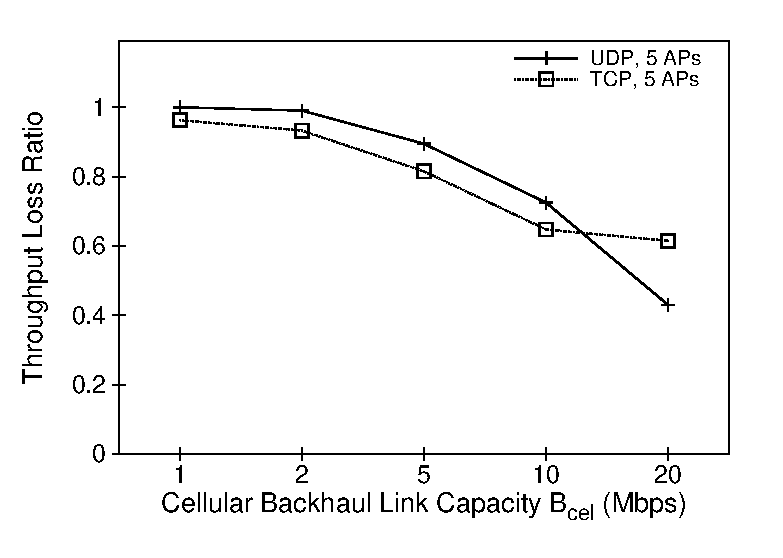
\includegraphics{./figures/eval/sim-sel-loss}}
       }
    \caption{Impact of selfish intensity on the performance of
	well-behaving nodes.}
    \label{fig:throughput-loss}
\end{figure}
%

%\subsubsection{Impact of Design Parameter}

%% Impact of B_{cel}
We next evaluate the impact of the backhaul link capacity $B_{cel}$ of
selfish tethering on the detection performance
for $B_{cel}$ = 2, 5, 10, and 20\! Mbps.
%
Fig.~\ref{fig:impact_bcel} shows the cumulative distribution of detection
time under various $B_{cel}$. The results indicate that more aggressive
selfish behavior, i.e., higher $B_{cel}$, is detected more quickly by
{\tt CUBIA} for both TCP and UDP protocols.
%
This indicates that {\tt CUBIA} can quickly detect aggressive selfish
behaviors, which is a very important design requirement for any good
detection scheme since such an aggressive behavior can seriously
degrade the performance of well-behaving nodes.
%
\begin{figure} [ht]
\center
  \subfigure[UDP]{
      \resizebox{41mm}{!}{
      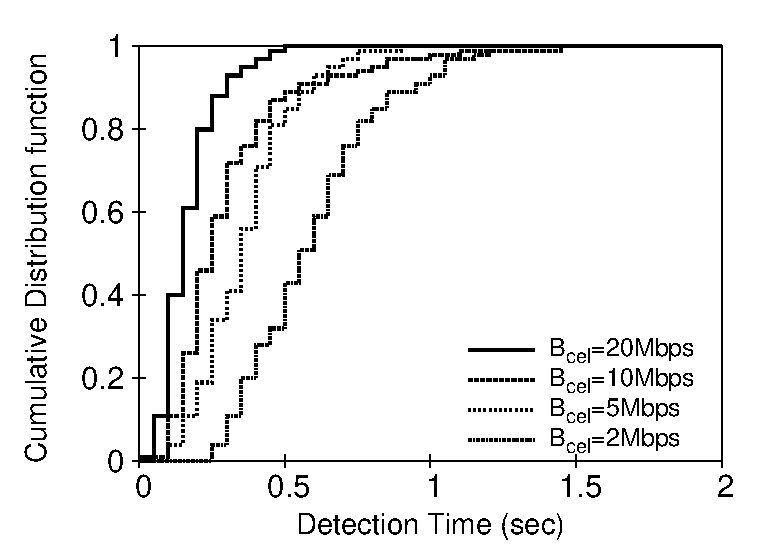
\includegraphics[]{./figures/eval/eval-CDF-detect-udp-M2}}
      }
  \subfigure[TCP]{
      \resizebox{41mm}{!}{
       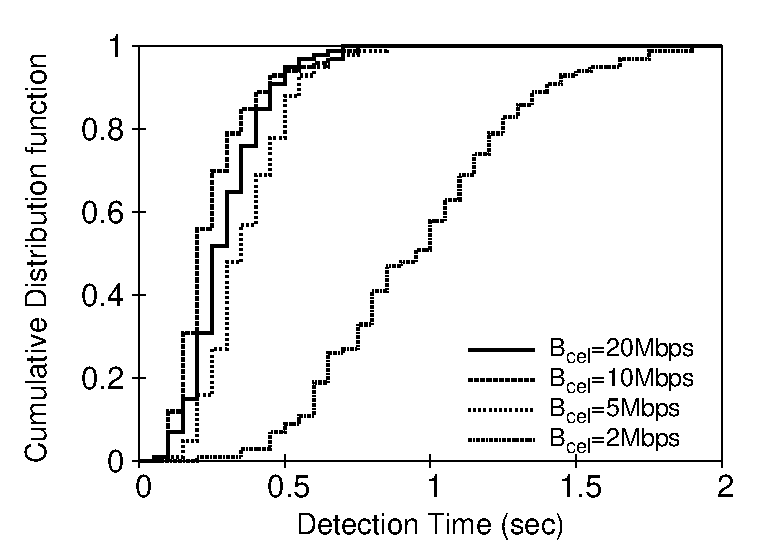
\includegraphics[]{./figures/eval/eval-CDF-detect-tcp-T2}}
       }
    \caption{Impact of $B_{cel}$ on detection time.}
    \label{fig:impact_bcel}
\end{figure}


Finally, we study the impact of alarm thresholds, i.e.,
$\theta_{AS}$ and $\theta_{S}$, on the detection time.
%
Fig.~\ref{fig:impact_threshold1} depicts the distribution of detection time
for 3 different values of the {\em first alarm threshold} $\theta_{AS}$.
%
It is straightforward that the use of a smaller value of $\theta_{AS}$ may
issue the first alarm too frequently and may incur an unnecessary overhead
for RTS/CTS exchange, resulting in the performance degradation. Meanwhile,
the results show that it takes less detection time with
a smaller $\theta_{AS}$.

Similarly, the impact of the {\em second alarm threshold} $\theta_{S}$
can be seen in Fig.~\ref{fig:impact_threshold2}. The figure compares
the detection time for different values of $\theta_{S}$ with
the given $\theta_{AS}$ = 3.
We can see that the detection time increases proportional to $\theta_{S}$.
However, there is a tradeoff between the false alarm ratio and
the detection time according to the choice of $\theta_{S}$.
For example, in case of the temporal behavior of the detection filter in
Fig.~\ref{fig-eval-dynamic3}, the use of a small value of $\theta_{S}$ can
cause false alarms (if $\theta_{S}$ is set to be less than $\theta_{AS}+1$,
it would issue several false alarms.)
although it can reduce the detection time unless the hidden node exists.
Thus, it is recommended to use a value of $\theta_{S}$ larger than
$\theta_{AS}+1$, to avoid false alarms
although it might take more time to detect.
%
\begin{figure} [ht]
\center
  \subfigure[UDP]{
      \resizebox{41mm}{!}{    \label{fig:impact_thresholdAS_UDP}
      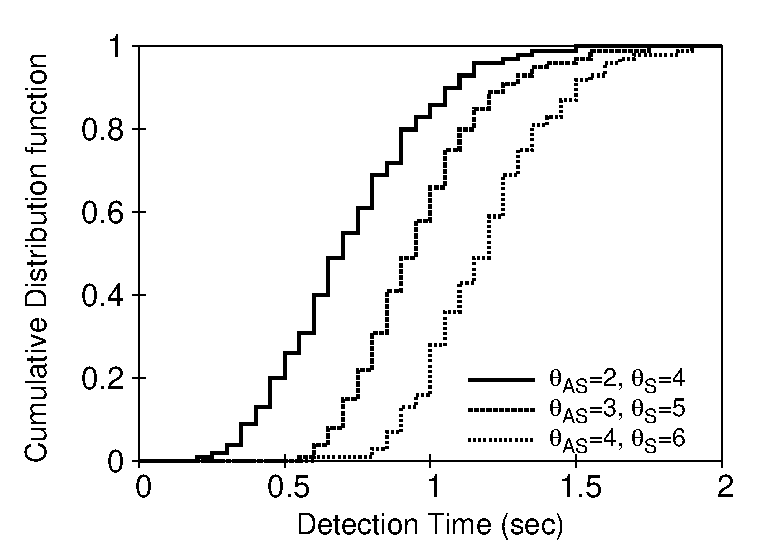
\includegraphics[]{./figures/eval/eval-CDF-impact_Tas-udp}}
      }
  \subfigure[TCP]{
      \resizebox{41mm}{!}{ \label{fig:impact_thresholdAS_TCP}
       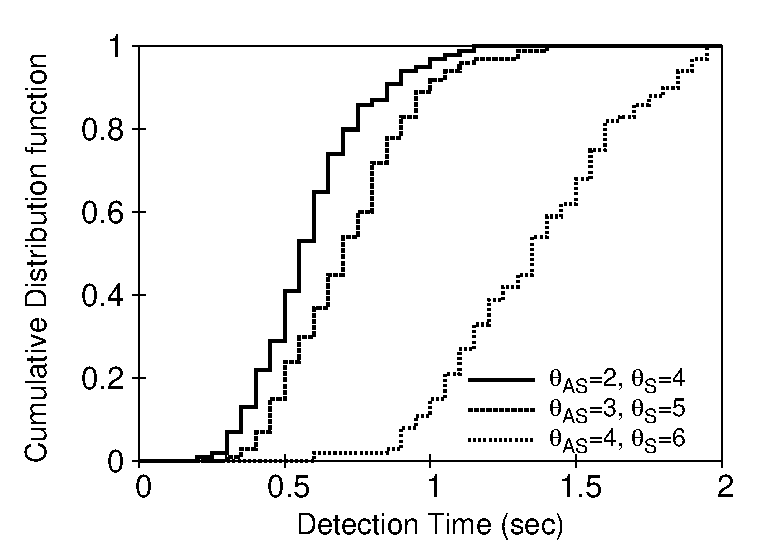
\includegraphics[]{./figures/eval/eval-CDF-impact_Tas-tcp}}
       }
    \caption{Impact of the first alarm threshold $\theta_{AS}$ on detection time
    for UDP and TCP protocols with $B_{cel}$\! =\! 20\! Mbps.}
    \label{fig:impact_threshold1}
\end{figure}
%
%
\begin{figure} [ht]
\center
  \subfigure[UDP]{
      \resizebox{41mm}{!}{    \label{fig:impact_thresholdS_UDP}
      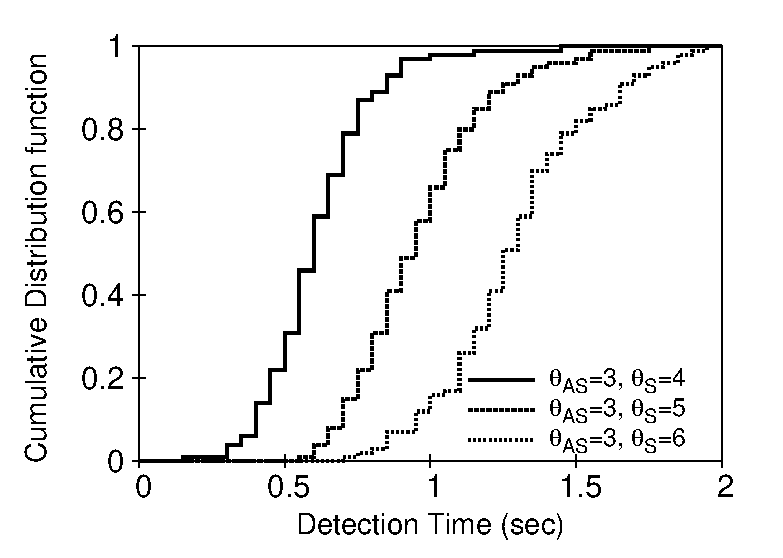
\includegraphics[]{./figures/eval/eval-CDF-impact_dT-udp}}
      }
  \subfigure[TCP]{
      \resizebox{41mm}{!}{ \label{fig:impact_threshold2S_TCP}
       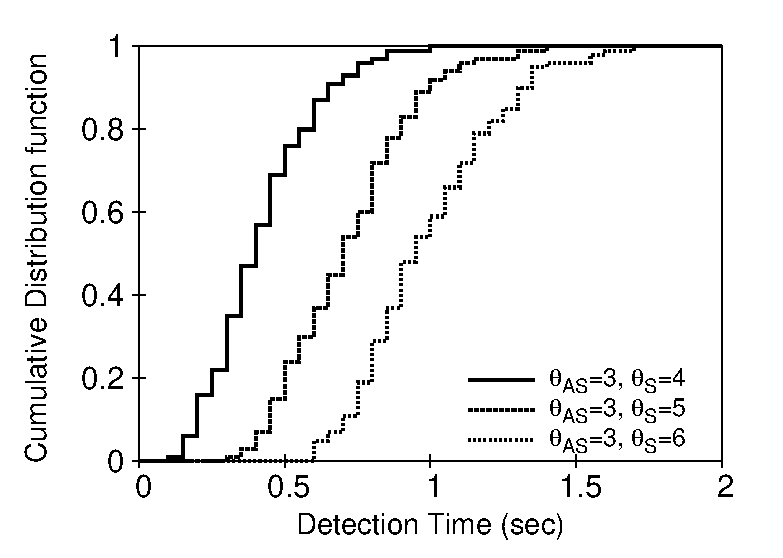
\includegraphics[]{./figures/eval/eval-CDF-impact_dT-tcp}}
       }
    \caption{Impact of the second alarm threshold $\theta_{S}$ for the given $\theta_{AS}$=3
    on detection time with $B_{cel}$\! =\! 20\! Mbps.}
    \label{fig:impact_threshold2}
\end{figure}

%\section{Related Work}

Selfish and malicious misbehavior in CSMA networks
has been extensively studied 
under various scenarios in different communication layers.
\cite{Kysanur:Vaidya05, Radosavac-Wise05, Raya-DOMINO, Toledo:Wang07a}.
%However,
%to the best of our knowledge, this is the first work that
%addresses the selfish misbehavior exploiting
%the Wi-Fi tethering environment.

%MAC-layer
Majority of previous work has concentrated on detecting or punishing
MAC-layer misbehavior \cite{Kysanur:Vaidya05, Raya-DOMINO, Radosavac-Wise05, Rong-Infocom06, Toledo:Wang07a}.
%
The authors of \cite{Kysanur:Vaidya05} have addressed the MAC layer misbehavior
selecting always small backoff values rather than random selection
and showed that such selfish misbehavior
can seriously degrade the performance of the network. To detect and penalize
the selfish misbehavior, they modified the MAC protocol and proposed a
receiver-side backoff allocation strategy where let
the receiver assign and send backoff values to the sender in
CTS and ACK frames.
Then, the assigned receiver uses them to detect potential misbehavior.
However, it needs to modification on the IEEE
802.11 protocol and the selfish receiver may exist.
%
In \cite{Radosavac-Wise05},
several possible misbehavior in 802.11 MAC protocol including
backoff manipulation are presented.
A detection framework, named DOMINO, considers
every possible strategies jointly and increases the detection accuracy.
The detection scheme for backoff manipulation is based on comparing
average values of the backoff to given thresholds.
However, this average metric is a suboptimal detection technique easily
misled by extremely large values of samples.
Some previous works~\cite{Toledo:Wang07a, Radosavac-Wise05} have utilized
statistical testing techniques such as
the Wald��s sequential probability ratio test~(SPRT)~\cite{Radosavac-Wise05},
Kolmogorov-Smirnov (K-S) test~\cite{Toledo:Wang07a}.
These works were important sources of inspiration for our work.
However, their operation cost is much higher
than our detection mechanism since their frameworks are
based on the comparison of distributions and
need to construct the probability distributions from
the observations. Moreover, no operational method to mitigate misbehavior
is proposed.


%Physical-layer
Some previous work has focused on routing layer misbehavior\cite{BenSalem03, Marti03}.
In 

% Routing-layer
Various solutions to routing layer misbehavior
(e.g., \cite{BenSalem03, Marti03})
and game theory-based approaches~\cite{MacKenzie01,Akella02} in wireless
ad hoc networks have been proposed.

%Multi-channel


%CCA Threshold





In our previous work,


A common way for a selfish user to increase his chance of accessing
the channel is to modify the operation of the 802.11 protocol
or change the MAC parameters related with
channel-attempt parameters, such as $CW_{min}$,
$CW_{max}$, and IFS~(inter-frame space).
Kyasanur and Vaidya \cite{Kysanur:Vaidya05} studied the MAC-layer misbehavior
of selecting always small backoff values rather than
random selection, and showed that such selfish misbehavior can
seriously degrade the network performance.
Raya {\em et al.}~\cite{Raya-DOMINO} investigated
multiple misbehavior policies in 802.11 MAC protocol including
backoff manipulations, and presented a detection framework, called DOMINO,
which considers all possible strategies jointly and improves the detection accuracy.
Recently, several statistic-based frameworks for detecting misbehavior
also have been introduced \cite{Radosavac-Wise05, Rong-Infocom06, Toledo:Wang07a}.
The common approach used in most prior works\cite{Kysanur:Vaidya05, Radosavac-Wise05,
Raya-DOMINO, Toledo:Wang07a} is to measure the inter-arrival time of target stations
in terms of the number of backoff slots and verify whether the backoff time of the stations follows a legitimate pattern or not.


Protocol misbehavior in 802.11 networks has been studied
in various scenarios in different communication layers.
The authors of \cite{Kysanur:Vaidya05} have addressed the MAC layer misbehavior
selecting always small backoff values rather than random selection
and showed that such selfish misbehavior
can seriously degrade the performance of the network. To detect and penalize
the selfish misbehavior, they modified the MAC protocol and proposed a
receiver-side backoff allocation strategy where let
the receiver assign and send backoff values to the sender in
CTS and ACK frames.
Then, the assigned receiver uses them to detect potential misbehavior.
However, it needs to modification on the IEEE
802.11 protocol and the selfish receiver may exist.
%
In \cite{Radosavac-Wise05},
several possible misbehavior in 802.11 MAC protocol including
backoff manipulation are presented.
A detection framework, named DOMINO, considers
every possible strategies jointly and increases the detection accuracy.
The detection scheme for backoff manipulation is based on comparing
average values of the backoff to given thresholds.
However, this average metric is a suboptimal detection technique easily
misled by extremely large values of samples.
Some previous works~\cite{Toledo:Wang07a, Radosavac-Wise05} have utilized
statistical testing techniques such as
the Wald��s sequential probability ratio test~(SPRT)~\cite{Radosavac-Wise05},
Kolmogorov-Smirnov (K-S) test~\cite{Toledo:Wang07a}.
These works were important sources of inspiration for our work.
However, their operation cost is much higher
than our detection mechanism since their frameworks are
based on the comparison of distributions and
need to construct the probability distributions from
the observations. Moreover, no operational method to mitigate misbehavior
is proposed.

% Routing-layer
Various solutions to routing layer misbehavior
(e.g., \cite{BenSalem03, Marti03})
and game theory-based approaches~\cite{MacKenzie01,Akella02} in wireless
ad hoc networks have been proposed. However, as the problem we
consider in this paper focuses on the MAC layer.

%Multi-channel

%%
The problem of misbehavior using CCA threshold is relatively new
and unexplored in the literature.
Recently, the authors~\cite{yang:choi-LCN09} have identified the effect of an
802.11 node's selfish behavior by increasing CCA threshold.
They have shown that the selfish behavior can achieve
higher throughput than other rational nodes based on
proposed game-theoretical model.
In \cite{Pelechris:Krish-Infocom09}, the selfish carrier sense problem
in WLANs was addressed. The authors have performed experimentation
on a real testbed and shown that such selfish behaviors can
cause extremely unfair allocations of the wireless medium.
We develop a detection scheme, named Carrier
sensing Misbehavior Detectio (CMD),
by exploiting power control mechanism.



%!TEX root = info-main.tex
\section{Conclusion and Future Work}
%
In this paper, we present {\tt CUBIA}, a novel Wi-Fi tethering misbehavior
detection mechanism that can accurately detect selfish behavior, e.g.,
manipulating CCA threshold, via AP-level collaboration in multi-AP
network environments.
%
We show that the benefits of MIM can be fully exploited and abused further
by a selfish tethering node via CCA manipulation combined with its short
link-distance.
%
We also observe that the consequence of the selfish tethering behavior resembles
that of the hidden node problem, but selfish tethering nodes tend to ignore
the RTS/CTS mechanism.
%
{\tt CUBIA} employs CUSUM algorithm for online detection of abnormal network
behavior and inject RTS/CTS frames to avoid mis-diagnosing the hidden node
problem as a selfish tethering.
%
Our simulation-based evaluation results show that {\tt CUBIA} accurately
distinguishes the selfish tethering behavior from other types of misbehavior
including the hidden node problem. 

In future, we would like to extend our work to pinpoint and localize
the selfish node based on the cooperation among APs.
It would also be interesting to study effective system-level follow-up 
actions against selfish tethering misbehavior, such as 
jamming-resilient dynamic channel re-assignment.

%To the best of our knowledge, this is the first attempt addressing the selfish
%node problem in a tethering environment. 


%\bibliographystyle{abbrv}
%\section*{Acknowledgment}

%The work reported in this paper was supported in part by the US NSF
%under Grant CNS-1160775.


%\bibliographystyle{abbrv}
\bibliographystyle{IEEEtran}
\begin{thebibliography}{1}

%A
\bibitem{Akella02}
A.~Akella, S.~Seshan, R.~Karp, and S.~Shenker,
``Selfish Behavior and Stability of the Internet: A Game-Theoretic Analysis of TCP,''
in {\em Proc. ACM SIGCOMM}, August 2002.

%B
\bibitem{Balasubramanian:09}
N. Balasubramanian, A. Balasubramanian, and A. Venkataramani,
``Energy Consumption in Mobile Phones: A Measurement
Study and Implications for Network Applications,''
{\em in Proc. ACM IMC}, November 2009.

\bibitem{BenSalem03}
N.~BenSalem, L.~Buttyan, J.P.~Hubaux, and M.~Jakobsson,
``A Charging and Rewarding Scheme for Packet Forwarding in Multihop Cellular Networks,''
in {\em Proc. ACM MobiHoc}, June 2003.

%C
\bibitem{Choi:Shin11}
J. Choi, and K. G. Shin,
``Out-of-band sensing with ZigBee for dynamic channel assignment
in on-the-move hotspots,''
{\em in Proc. IEEE ICNP}, October 2011.

\bibitem{choi:shin12}
J. Choi, and K. G. Shin,
``QoS provisioning for large-scale multi-AP WLANs,''
{\em Elsevier Ad-hoc Networks}, vol. 10, no. 2, pp. 174-185, March 2012.

\bibitem{Cisco:13}
Cisco, ``{Cisco Visual Networking Index: Global Mobile Data Traffic Forecast
  Update, 2012-2017},'' February 2013.

%D
\bibitem{Himanshu2010}
H. Dwivedi, C. Clark, and D. Thiel,
{\em Mobile application security}, McGraw-Hill Education, 2010.

%E

%F

%G
\bibitem{FIM08}
M.~Garetto, T.~Salonidis, and E. W. Knightly,
``Modeling per-flow throughput and capturing starvation in csma multi-hop wireless networks,''
{\em IEEE/ACM Trans. Netw.}, vol. 16, no. 4, pp. 864-877, August 2008.

\bibitem{Gustafsson:2000}
F.~Gustafsson,
\newblock {Adaptive filtering and change detection}.
\newblock {\em John Wiley \& Sons, Ltd}, 2000.

%H

%I

%J
\bibitem{Jensen10}
T.~Jensen, S.~Kant, J.~Wehinger, and B.~Fleury,
``Fast link adaptation for MIMO OFDM,''
{\em IEEE Trans. Veh. Tech.}, vol. 59, no. 8, pp. 3766-3778, October 2010.

\bibitem{Joshi:Katti2013}
K.~Joshi, S.~Hong and S.~Katti
``PinPoint: Localizing interfering radios''
{\em in Proc.} 10th USENIX NSDI, April 2013.

%K
\bibitem{CARA}
J. Kim, S. Kim, S. Choi, and D. Qiao,
``CARA: Collision-aware rate adaptation for ieee 802.11 WLANs,''
{\em in Proc. } IEEE INFOCOM, April 2006.


\bibitem{K:Vaidya05}
P.~Kyasanur and N.H.~Vaidya,
``Selfish MAC layer misbehavior in wireless networks,''
{\em IEEE Trans. Mob. Comp.}, vol. 4, no. 5, pp. 502-516, September/October 2005.

%L
\bibitem{jlee:ychoi07}
J. Lee, W. Kim, S.~Lee, D.~Jo, J.~Ryu, T.~T.~Kwon, and Y.~Choi,
``An experimental study on the capture effect in 802.11a networks,''
{\em in Proc. } ACM WinTECH, August 2007.

\bibitem{capture}
K. Leentvaar and J. Flint,
``The capture effect in FM receivers,''
{\em IEEE Trans. on Comm.}, vol. 24, no.5, pp. 531-539, May 1976.

%M
\bibitem{MacKenzie01}
A.~MacKenzie and S.~Wicker,
''Game theory and the design of selfconfiguring, adaptive wireless networks,''
{\em IEEE Commun. Mag.}, vol. 39, no. 11, pp. 126-131, November 2001.


\bibitem{Marti03}
S.~Marti, T.J.~Giuli, K.~Lai, and M.~Baker,
``Mitigating Routing Misbehavior in Mobile Ad Hoc Networks,''
in {\em Proc. ACM MobiCom}, August 2000.


\bibitem{MIM}
J. Manweiler, N. Santhapuri, S. Sen, R. R. Choudhury, S. Nelakuditi,\, and\, K. Munagala,
``Order matters:\,Transmission reordering in wireless networks,''
{\em IEEE/ACM Trans. on Net. (ToN)}, vol. 20, no. 2, pp. 353-366, April 2012.

\bibitem{Mishra_MC2R_2005}
A. Mishra, S. Banerjee, and W. Arbaugh,
``Weighted coloring based channel assignment for WLANs,''
{\em Mobile Computer Communications Review (MC2R)}, vol. 9, no. 3, pp. 19-31, July 2005.

\bibitem{client_driven06}
A. Mishra, V. Brik, S. Banerjee, A. Srinivasan, and W. Arbaugh.
``A client-driven approach for channel management in wireless LANs,''
{\em in Proc.} IEEE INFOCOM, April 2006.

\bibitem{Mishra:Arbaugh05}
A.~Mishra, E.~Rozner, S.~Banerjee, and W.~Arbaugh,
``Exploiting partially overlapping channels in wireless networks: Turning a peril into an advantage,''
{\em in Proc.} ACM/USENIX IMC, October 2005


\bibitem{Mishra_06}
A. Mishra, V. Shrivastava, D. Agarwal, and S. Banerjee,
``Distributed channel management in uncoordinated wireless environments,''
{\em in Proc.} ACM MOBICOM, September 2006.
%N

%O

%P
\bibitem{Pelechris:Krish-Infocom09}
K.~Pelechrinis, G.~Yan, S.~Eidenbenz, and S.~V.~Krishnamurthy,
``Detecting Selfish Exploitation of Carrier Sensing in 802.11 Networks,''
{\em in Proc.} IEEE INFOCOM, April 2009.

%Q

%R
\bibitem{Radosavac-Wise05}
S. Radosavac, J. Baras, and I. Koutsopoulos,
``A framework for MAC protocol misbehavior detection in wireless networks,''
{\em in Proc.} ACM WiSe, September 2005.

\bibitem{Raya-DOMINO}
M.~Raya, I.~Aad, J.-P.~Hubaux, and A.~E.~Fawal,
``DOMINO: Detecting MAC layer greedy behavior in IEEE 802.11 hotspots,''
{\em IEEE Trans. Mobile Comp.}, vol. 5, no. 12, pp. 1691-1705, December 2006.

%S

%T

\bibitem{Tang:Zhuang13}
J. Tang, and Y. Cheng,
``Selfish Misbehavior Detection in 802.11 Based Wireless Networks:
An Adaptive Approach Based on Markov Decision Process,''
{\em in Proc.} IEEE INFOCOM, April 2013.

\bibitem{Toledo:Wang07a}
A.~Toledo, and X.~Wang,
``Robust Detection of Selfish Misbehavior in Wireless Networks,''
{\em IEEE Journal on Selected Areas in Communications}, vol. 25, no. 6,
pp. 1124-1134, August 2007.

\bibitem{Tse:Viswanath05}
D. Tse and P. Viswanath,
\emph{Fundamentals of Wireless Communications}.
Cambridge University Press, 2005.

%U

%V

%W
\bibitem{Ware:Dut00}
C. Ware, J. Judge, J. Chicharo, and E. Dutkiewicz,
``Unfairness and capture behaviour in 802.11 adhoc networks,''
{\em in Proc.} IEEE ICC, June 2000.

%X
\bibitem{yang:choi-LCN09}
E.~Yang, J.~Choi, and S.~Lee,
``On selfish behavior using asymmetric carrier sensing in IEEE 802.11 wireless networks,''
{\em in Proc.} IEEE LCN, October 2008.

%Z
\bibitem{zhang:shin11icnp}
X.~Zhang and K. G. Shin,
``Adaptive subcarrier nulling: Enabling partial spectrum sharing in wireless lans,''
{\em in Proc. } IEEE ICNP, October 2011.

\bibitem{Zhang:Lazos13}
Y.~Zhang and L.~Lazos,
``Countering Selfish Misbehavior in Multi-channel
MAC Protocols,''
{\em in Proc.} IEEE INFOCOM, April 2013.
%ETC
\bibitem{NS2}
\newblock {The Network Simulator-ns2,}
www.isi.edu/nsnam/ns.

\bibitem{Wigle}
\newblock {Wiggle: Wireless geographic logging engine,}
http://www.wigle.net/.

\bibitem{Android}
\newblock {Google Android,}
http://www.android.com/.


% PCworld2011 : http://www.pcworld.com/article/228078/how_does_atandt_detect_jailbreak_tethering.html

\end{thebibliography}


% biography section
%
% If you have an EPS/PDF photo (graphicx package needed) extra braces are
% needed around the contents of the optional argument to biography to prevent
% the LaTeX parser from getting confused when it sees the complicated
% \includegraphics command within an optional argument. (You could create
% your own custom macro containing the \includegraphics command to make things
% simpler here.)
%\begin{biography}[{\includegraphics[width=1in,height=1.25in,clip,keepaspectratio]{mshell}}]{Michael Shell}
% or if you just want to reserve a space for a photo:

%\begin{IEEEbiography}{Michael Shell}
%Biography text here.
%\end{IEEEbiography}

% if you will not have a photo at all:
%\begin{IEEEbiographynophoto}{John Doe}
%Biography text here.Biography text here.Biography text here.Biography text here.Biography text
%\end{IEEEbiographynophoto}

% insert where needed to balance the two columns on the last page with
% biographies
%\newpage

% You can push biographies down or up by placing
% a \vfill before or after them. The appropriate
% use of \vfill depends on what kind of text is
% on the last page and whether or not the columns
% are being equalized.

%\vfill

% Can be used to pull up biographies so that the bottom of the last one
% is flush with the other column.
%\enlargethispage{-5in}

% that's all folks
\end{document}



